\usepackage{here}
\usepackage{listings}
\usepackage{color}
\definecolor{dkgreen}{rgb}{0,0.6,0}
\definecolor{gray}{rgb}{0.5,0.5,0.5}
\definecolor{mauve}{rgb}{0.58,0,0.82}

\lstset{
language={Ruby},
basicstyle={\small},
identifierstyle={\small},
commentstyle={\small\itshape\color{dkgreen}},
keywordstyle={\small\bfseries\color{blue}},
ndkeywordstyle={\small},
stringstyle={\small\ttfamily\color{mauve}},
frame={tb},
breaklines=true,
columns=[l]{fullflexible},
numbers=left,
xrightmargin=0zw,
xleftmargin=3zw,
numberstyle={\scriptsize},
stepnumber=1,
numbersep=1zw,
lineskip=-0.5ex
}


\title{集合知の成功事例としての株価変動についての調査}
\author{プロジェクトマネジメントコース\\
ソフトウェア開発管理グループ\\
矢吹研究室\\
1242109\\
三宅琢己}
\date{}
\begin{document}
\maketitle

%本テンプレートの余白は,卒論マニュアルで指示されたものとは違っているが,1ページあたりの文字数は40文字x40行と,卒論マニュアル通りになっている。文字間隔や行間隔を調整して,余白をマニュアル通りにすることもできるが,それでは文章が読みにくくなるため,このような対応をしている。

%\noindent
□□□□□□□□□■□□□□□□□□□■□□□□□□□□□■□□□□□□□□□■
□□□□□□□□□■□□□□□□□□□■□□□□□□□□□■□□□□□□□□□■
□□□□□□□□□■□□□□□□□□□■□□□□□□□□□■□□□□□□□□□■
□□□□□□□□□■□□□□□□□□□■□□□□□□□□□■□□□□□□□□□■
□□□□□□□□□■□□□□□□□□□■□□□□□□□□□■□□□□□□□□□■
□□□□□□□□□■□□□□□□□□□■□□□□□□□□□■□□□□□□□□□■
□□□□□□□□□■□□□□□□□□□■□□□□□□□□□■□□□□□□□□□■
□□□□□□□□□■□□□□□□□□□■□□□□□□□□□■□□□□□□□□□■
□□□□□□□□□■□□□□□□□□□■□□□□□□□□□■□□□□□□□□□■
□□□□□□□□□■□□□□□□□□□■□□□□□□□□□■□□□□□□□□□■
□□□□□□□□□■□□□□□□□□□■□□□□□□□□□■□□□□□□□□□■
□□□□□□□□□■□□□□□□□□□■□□□□□□□□□■□□□□□□□□□■
□□□□□□□□□■□□□□□□□□□■□□□□□□□□□■□□□□□□□□□■
□□□□□□□□□■□□□□□□□□□■□□□□□□□□□■□□□□□□□□□■
□□□□□□□□□■□□□□□□□□□■□□□□□□□□□■□□□□□□□□□■
□□□□□□□□□■□□□□□□□□□■□□□□□□□□□■□□□□□□□□□■
□□□□□□□□□■□□□□□□□□□■□□□□□□□□□■□□□□□□□□□■
□□□□□□□□□■□□□□□□□□□■□□□□□□□□□■□□□□□□□□□■
□□□□□□□□□■□□□□□□□□□■□□□□□□□□□■□□□□□□□□□■
□□□□□□□□□■□□□□□□□□□■□□□□□□□□□■□□□□□□□□□■
□□□□□□□□□■□□□□□□□□□■□□□□□□□□□■□□□□□□□□□■
□□□□□□□□□■□□□□□□□□□■□□□□□□□□□■□□□□□□□□□■
□□□□□□□□□■□□□□□□□□□■□□□□□□□□□■□□□□□□□□□■
□□□□□□□□□■□□□□□□□□□■□□□□□□□□□■□□□□□□□□□■
□□□□□□□□□■□□□□□□□□□■□□□□□□□□□■□□□□□□□□□■
□□□□□□□□□■□□□□□□□□□■□□□□□□□□□■□□□□□□□□□■
□□□□□□□□□■□□□□□□□□□■□□□□□□□□□■□□□□□□□□□■
□□□□□□□□□■□□□□□□□□□■□□□□□□□□□■□□□□□□□□□■
□□□□□□□□□■□□□□□□□□□■□□□□□□□□□■□□□□□□□□□■
□□□□□□□□□■□□□□□□□□□■□□□□□□□□□■□□□□□□□□□■
□□□□□□□□□■□□□□□□□□□■□□□□□□□□□■□□□□□□□□□■
□□□□□□□□□■□□□□□□□□□■□□□□□□□□□■□□□□□□□□□■
□□□□□□□□□■□□□□□□□□□■□□□□□□□□□■□□□□□□□□□■
□□□□□□□□□■□□□□□□□□□■□□□□□□□□□■□□□□□□□□□■
□□□□□□□□□■□□□□□□□□□■□□□□□□□□□■□□□□□□□□□■
□□□□□□□□□■□□□□□□□□□■□□□□□□□□□■□□□□□□□□□■
□□□□□□□□□■□□□□□□□□□■□□□□□□□□□■□□□□□□□□□■
□□□□□□□□□■□□□□□□□□□■□□□□□□□□□■□□□□□□□□□■
□□□□□□□□□■□□□□□□□□□■□□□□□□□□□■□□□□□□□□□■
■■■■■■■■■■■■■■■■■■■■■■■■■■■■■■■■■■■■■■■■
□□□□□□□□□■□□□□□□□□□■□□□□□□□□□■□□□□□□□□□■%文字数チェック用
\tableofcontents%目次
\chapter{序論}

\section{研究背景}

1986年スペースシャトル・チャレンジャー号爆発事故が起きた.
その直後,事故に関連していた4社の株価が急落した.そのうち3社の株価は持ち直したのだが,1社の株価だけさらに下がり,持ち直すことはなかった.
この事故の原因は明らかになっていないのにも関わらず,このような株価の変動が起きた.

その数か月後,その1社の部品が原因で爆発事故が起きたことを公表した\cite{miyake2}.

この結果だけ見ると株式市場は原因企業を特定していたのではないかと考えられる.

株式市場は賢く,原因企業を本当に特定していたのか,それとも偶然このようなことが起きたのか.



\section{研究背景となった話}


1986年1月28日午前11時38分,スペースシャトルチャレンジャー号がフロリダ州ケーブカナベラルから発射された.74秒後,チャレンジャー号は地表から16キロ上空まで上昇し,そして爆発した.

その発射の模様はテレビ中継されていたので,事故のニュースは素早く伝わり,爆発から8分後,ダウジョーンズ・ニューズワイヤーズが最初の報道をした.

株式市場は最初の報道から数分もしないうちにチャレンジャー号発射にかかわった主要企業4社の株を投売り始めた.

\begin{itemize}
  \item ロックウェルインターナショナル

シャトルとメインのエンジン担当
  \item ロッキード

地上支援担当
  \item マーティン・マリエッタ

シャトルの外部燃料タンク担当
  \item モートン・サイオコール  

固体燃料ブースター担当
\end{itemize}


爆発から21分後,ロッキードの株価は5パーセント,マーティン・マリエッタの株価は3パーセント,ロックウェルの株価は6パーセント下落していた.

だが,一番下落幅が大きかったのはモートン・サイオコールの株価であった.

チャレンジャー号の賛辞をめぐる市場の反応については,ファイナンスの教授であるマイケル・T・マロニーとJ・ハロルド・マルヘリンの2名の手になる
すばらしい研究がある.

サイオコール株を売りたい投資家があまりに多かった一方で,買いたい投資家があまりに少なかったために,同株は瞬く間に取引停止に追い込まれた.
爆発からほぼ1時間後に売買が再開されたとき,株価は6パーセント下落し,その日の終値では下落幅が約12パーセントだった.

対照的に,残りの3社の株価は持ち直して,下落幅は2パーセント程度にとどまった.
これは,ほぼ瞬時に株式市場がチャレンジャー爆発の原因はモートン・サイオコールにあり,
この惨事が同社のボトムラインに与える影響は深刻だと判断したことを示す確たる証拠である.

理論的に言えば株式市場は,企業が将来獲得するすべてのフリーキャッシュフローの現在価値を計算するメカニズムであるとされている
(フリーキャッシュフローとは,企業が経費や税金を支払い,減価償却や投資をした後に残るお金である.自分がその企業のたった一人の株主なら,
持ち帰って自分の口座に貯金できるお金とも言い換えられる).

マロニーとマルヘリンが指摘するように,事故の当日,サイオコールに責任があるというコメントは1つとして公になっていなかった.

明くる朝,ニューヨークタイムズ紙に掲載された記事は当時出回っていた2つの噂に言及したが,いずれもサイオコールに責任があることをうかがわせる内容ではなかった.
同氏は「事故の原因を特定する手がかりはない」と断言している.

だが,市場は正しかった.

爆発から6か月後,チャレンジャー号大統領調査委員会は低温のせいでサイオコール製のブースターロケットに取り付けられたOリングシールの弾力性が失われ,隙間ができたためにガス漏れが起きたこと明らかにした.Oリングシールは燃焼ガスの漏れを防ぐための部品だが,チャレンジャーの事故ではOリングシールから漏れた燃焼ガスがメインの燃料タンクを燃やして大爆発を引き起こした.
それにより,サイオコールの責任が認められ,他社の嫌疑が晴れた.

市場がサイオコールを選び出したのは,単なる偶然だったのかもしれない.たまたま同社の事業が宇宙開発計画の中断を受けやすい,と思われただけかもしれない.あるいは取引停止という事態が,投資家に何かのメッセージを送ったのかもしれない.

こういう点にも注意すべきではあるが,この時の市場の動きは不思議だったとしか言いようがない.

一般的に株式市場はメディアの憶測やウォールストリートの狂乱などに歪められることが多く,個々の投資家の知恵を集約して集団の知恵を得るメカニズムとしては不安定である.それにもかかわらず,あの日の株式市場が純粋な計算機械としてきちんと機能したということが何とも不思議なのである.

市場はどうやって正しい意見にたどり着いたのだろうか.
マロニーとマルヘリンをてこずらせたのがこの問いである.

自社に責任があると知っていたサイオコールの幹部が1月28日に株を投売りしたかもしれないと考え,インサイダー取引を示す証拠を探した.
でもそんな証拠は見つからなかった.

Oリングについて知っていたライバル企業の幹部が,サイオコールの株を投売りして,残りの3社の株を買いあさった人もいなかった.

抜け目ないインサイダーのせいで,事故当日のサイオコールの株価が下落したのではない.比較的手持ちの情報の少ない投資家が,同社の株を買わなかっただけのことだった.

では,「どうして誰もサイオコールの株を買いたくなかったのだろうか」.

この問いに対してマロニーとマルヘリンは最後まで説得力のある答えを見つけられなかった.
コーネル大学の経済学者であるモーリーン・オハラの含蓄のある言葉を引用した,

「市場は実践的にはうまく機能しているように見えるが,実際にどのように機能しているか理論的には不明である」.

オハラの言葉ももっともだが,それはたぶん「理論」という言葉の定義にもよる.

あの日の出来事をごくごく単純化すると,次のようになる.

特に関係もない多数の個人の集まりが,「チャレンジャーが爆発してしまったいま,この4社の企業価値はどれほど下がっただろうか」という,
客観的に正しい答えが存在する問いを突き付けられた.
ここに集団の平均的な予測値,この場合は金額加重の株価予測の確度が高くなる要件が隠されている.Oリングに関するインサイダー情報を知っている人がいた可能性は否定できない.だが,そんな人がいたかどうかに関係なく,その日一人ひとりのトレーダーの頭の中にあった事故に関する情報のかけらを足し集めたら,真相に近いものが生まれる可能性も十分ある.

サイオコールと事故の関係について確かなことを知っている個人は存在していなくても,確かなことを知っている集団は存在していたのだ.

この日,市場が賢い判断を下せたのは,賢い集団の4つの要件が満たされていたからだ.
\begin{itemize}
  \item 意見の多様性

それが既知の事実のかなり突拍子もない解釈だとしても,各人が独自に私的情報を多少なりと持っている
  \item 独立性

他者の考えに左右されない
  \item 分散性

身近な情報に特化し,それを利用できる
  \item 集約性  

個々人の判断を集約して集団として1つの判断に集約するメカニズムの存在
\end{itemize}


この4つの要件を満たした集団は,正確な判断が下しやすい.
なぜか.
多様で,自立した個人から構成される,ある程度の規模の集団に予測や推測をしてもらってその集団の回答を均すと,一人ひとりの個人が回答を出す過程で犯した間違いが相殺される.

言ってみれば,個人の回答には情報と間違いという2つの要素がある.算数のようなもので,間違いを引き算したら情報が残るというわけである.
「集団の知恵」という言葉に実質の伴った価値を与え,私たちを驚かせてやまないのは,みんなの意見に含まれている情報量の多さである.

チャレンジャーの事故のケースでは,集団が共有する集合的な「頭」の中に世界のほぼ完璧な絵が描かれている\cite{miyake2}.



\chapter{研究目的}


背景にあることを調査するためには,銘柄・期間を指定し,さらに株価データの変動を可視化できるようにする必要がある.
そのようなことを可能にするツールの開発を本研究での目的とする.

完成次第背景にある,株式市場は賢いのか,そうでもないのかを進めるものとする.


株価データの取得方法はRubyによるクローラーで取得する.
ネット上には膨大な情報量がある中で,自分から必要な情報を引っ張り出す必要がある.
その勉強をするためにこのような株価データの取得方法をとる.

         


	                                                                                 




\chapter{集合知とは}

集合知というのはナレッジマネジメントの分野ではもともとの意味は複数人の智恵の集合と言う意味である.
開発や課題解決に取り組む時,天才的な超優秀な一人より,それなりに優秀な何人かの集合が,複数の視点を上手に使って取り組む方が高い成果を生むことができる場合もあるということ.

議論の中で様々な意見が飛び交う中でよりよいアイディアや意見が生まれる.

\section{集合知収集の4つの手順}
集合知を収集しやすくするためには以下の4つの手順通り進める必要がある.
\begin{enumerate}
  \item 公開

情報を原則的には私物化せず,すべて公開する.

  \item 連鎖

情報と情報を指標に基づき関連付けて,新たな意見,発想へと展開する.

  \item 選別

必要な情報であるか,そうでないかを選別し,必要な情報のみを管理するようにする.
  \item 評価

公開されている情報をコメントなどにより評価し,情報に優先順位をつける.




\end{enumerate}


\chapter{ナレッジマネジメントとは}
企業経営における管理領域の一つ.生産管理,販売管理,財務管理,人的資源管理,情報管理に続く第6の管理領域.
個人のもつ暗黙知を形式知に変換することにより,知識の共有化,明確化を図り,作業の効率化や新発見



を容易にしようとする企業マネジメント上の手法である\cite{management}.

\section{SECIモデル}
「個人の知識を組織的に共有し,より高次の知識を生み出す」ということを主眼に置いたナレッジマネジメントを実現する場合,そのフレームワークとして以下の4段階のプロセスが提示されている.

このプロセスは,各段階の英語名称の頭文字をとってSECI(セキ)プロセス,あるいは単にSECI(セキ)と呼ばれる.
これは野中郁次郎(一橋大学 名誉教授)と竹内弘高(ハーバード大学ビジネススクール 教授一橋大学 名誉教授)が執筆したThe Knowledge Creating Company(『知識創造企業』梅本勝博訳,東洋経済新報社)において,提唱された.知識とは「正当化された真なる信念 (Justified true belief)」であり,個人と個人の相互作用、あるいは組織と組織の相互作用により,ダイナミックに変化・深化・進化していくものであるという考えの下に構築されている.

SECIモデルは以下の頭文字をとったものである.
\begin{itemize}
  \item 共同化(Socialization)暗黙知から暗黙知へ

組織内の個人,または小グループでの暗黙知共有,およびそれを基にした新たな暗黙知の創造である.

  \item 表出化(Externalization)暗黙知から形式知へ

各個人,小グループが有する暗黙知を形式知として洗い出すこと.
  \item 結合化(Combination)形式知から形式知へ

洗い出された形式知を組み合わせ,それを基に新たな知識を創造することである.
  \item 内面化(Internalization)形式知から暗黙知へ

新たに創造された知識を組織に広め,新たな暗黙知として習得することである\cite{management}.

\end{itemize}

\begin{figure}[H]
\centering
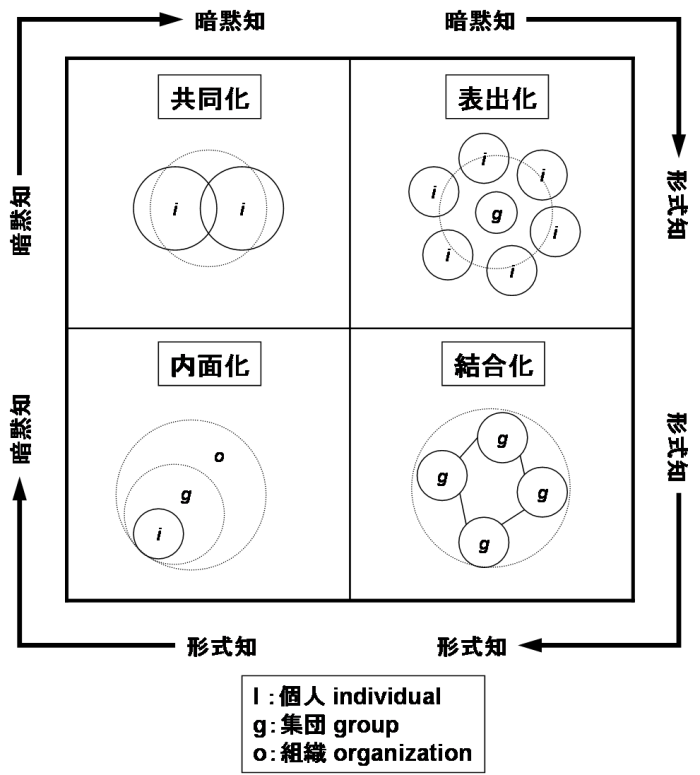
\includegraphics[width=15cm]{SECI_pro.PNG}
\caption{SECIプロセス}\label{サンプル図}
\end{figure}


\section{具体的な手法}
主に以下の手法があるが,それぞれ独立したものでなく,相互依存的なものである\cite{management}.
\subsection{データマイニング}
人工知能や統計学を利用してデータから知識を取り出そうとする試み.主に共起現象を探り,セールスに結びつけようとしている.

\begin{itemize}
  \item 例1:スーパーでビデオとガムが共に売れる→両者を同じ場所に置く.
  \item 例2:本Aを買う人は,後に本Bを買うことが多い→購入者に本Bを薦めるダイレクトメールを送る.
  \item 従来の統計学と大差ないが,POSやオンラインショッピングによる大量のITデータの中から法則性を見つけ出すことに主眼が置かれている\cite{management}.
\end{itemize}

\subsection{データウェアハウス}
データを多次元的に処理することにより,通常では察知しにくい傾向性を発見する技法.多次元データベースなど,幾つもの次元によって処理が可能なソフトウェアが開発されている.

\begin{itemize}
  \item 例:時間,空間,取り扱い物によって販売量が明示される → 時系列や地域、取り扱い物の傾向が分かる\cite{management}.
\end{itemize}

\subsection{知識共有化}
電子掲示板やメーリングリスト,知識ベース,オンラインコラボレーションなどを使って,一部の人の資産であった知識の,集団全体への共有を図るもの.
基本的には文字や印刷といったメディアの問題であるが,電子通信技術の一新によって,電子メール・電子掲示板に代表されるような新しい共有化のあり方が模索されている.
具体的には,企業内ではグループウェアなどを使って知識共有の試みが行われることが多い.インターネット上でも,OKWave,はてなのように広範な分野を扱うサイトや,Apple Support Discussionのような特定者向けサイトによる知識共有化の試みが始まっている.
近年,エンタープライズ2.0と呼ばれる大企業での情報共有が積極的に行われるようになってきた\cite{management}.


\subsection{可視化}
人間における視覚の優位性を利用し,多次元・多要素で理解しにくい情報を,見える形で表現し,理解しやすくさせること.
原理的にはグラフや図画であるが,ナレッジマネジメントではCGを利用した立体的で動的な画像を使って表現するケースが多い.


様々な手法はあるものの,通常の技法と同じく,それを使いこなすのは熟練と才能が必要とされるため,電子メールやQA知識ベースなどいくつかを除けば,実際に有効活用されている例は少ない.
また暗黙知を明示化するには原理的に大きな困難が伴うため,共有化された知識はあまり役に立たない常識的なものがほとんどで,実際にほしい熟練した技能や知恵は掘り出せないことが多いため,研究自体は尻すぼみになっている\cite{management}.

\subsection{エンタープライズサーチ}
企業組織内の書類,人事,経営情報等を検索できるようにするためのシステム,またはそのコンセプトのこと\cite{management}.


\section{知識変換の「場」}
組織として,知識の創造,共有,活用,蓄積を活発化させるために,個々のナレッジを共有したり,共同でナレッジを創造したりするための結節点が必要となる.この結節点を,「場」と言う.豊かな知識創造・知識経営が出来るかどうか,「場」のデザインにかかってくる.「場」は,SECIモデルの各フェーズに沿って,4つのパターンに分けることができる\cite{ba}.


\subsection{創発場(Originating Ba)}
\begin{itemize}
  \item 共同化に対応
\end{itemize}

経験,思い,信念,考え方などの暗黙知を共有する場である\cite{ba}.

\subsection{対話場(Dialoguing Ba)}
\begin{itemize}
  \item 表出化に対応
\end{itemize}

各自が対話(ダイアローグ)を通じて暗黙知を言語化・概念化して形式知に変換するための場である\cite{ba}.

\subsection{システム場(Systemizing Ba)}
\begin{itemize}
  \item 結合化に対応
\end{itemize}

形式知を相互に移転・共有・編集・構築し,新たな体系の形式知へと統合する場である\cite{ba}.

\subsection{実践場(Exercising Ba)}
\begin{itemize}
  \item 内面化に対応
\end{itemize}

形式知を個々人の暗黙知へと身体化するための場である.ここでは,単なる形式知の伝達ではなく,形式知に束ねる形で何らかの経験的要素や人間的要素を提供することで暗黙知としての移転・発展を促すことができる.サービス業などで特に重要な場である\cite{ba}.

\begin{figure}[H]
\centering
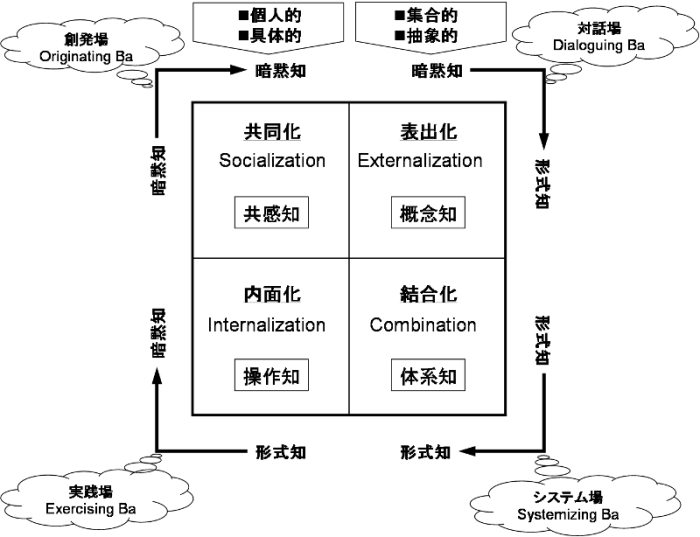
\includegraphics[width=15cm]{SECI_ba.PNG}
\caption{SECIプロセスの「場」について}\label{サンプル図}
\end{figure}

\chapter{株とは}
\section{株とは}
企業が事業資金を調達するために,発行しているものである.企業は,投資家が株を買ってくれた資金等を使って事業を拡大する.
「株を買う」ということは,株を発行している企業に出資を行い,事業資金を提供していることを意味する.

まとめると,株とは,
「株を買う(株主になる)」=「出資者になる」=「会社のオーナーの一人になる」
ことを意味する\cite{kaisya}.

また,株の大きな特徴として,買った株を第三者に転売することができる.株を転売すれば,会社のオーナー(株主)の権利等は,新しいオーナー(株主)に移ることになる\cite{kabu}.

\section{株式会社とは}
細分化された社員権(株式)を有する株主から有限責任の下に資金を調達して株主から委任を受けた経営者が事業を行い,利益を株主に配当する,法人格を有する企業形態である.このような企業形態は各国で見られる.

\section{株価変動の要因}
株価変動の要因はさまざまである.

上昇の要因と下落の要因を説明する.

\subsection{株価上昇の要因}
基本的に株が上がって行く状態というのは,買い手が多い,つまりはその株は人気が高い状態にあるよいうことである.
\begin{enumerate}
  \item 業績が好調である

業績が好調であるということは,利益を生み出しやすい状態にあるということである.投資家から人気が高いのは当然である.
  \item 業績の見通しを上方修正した

当初の会社の予想より,見通しを上方修正した時である.会社側が思っていたよりも利益が出そうという報告である.これも好感される.
 \item 復配・増配をする

今期は配当金を出す,または前回より配当金を増やすと発表した時である.復配や増配は,業績が好調の証であるため,投資家に好感されることがある.
  \item 新製品の発表・新しい工場の建設など

新しいことを始めるのは,リスクももちろんあるが,利益を増やすために行うものである.これにより利益が増えるという判断をされた場合には,株価が上がる.
  \item 合併・買収

企業の合併・買収により,企業間の相乗効果が出て,企業価値が上がると判断された場合には,株価が上がる.
  \item 割安株の修正

割安に放置されていた株が,とある出来事をきっかけに株価上昇が起きることがある.とある出来事というのは,上の1~5の理由もそうであるし,東証2部から東証1部へ移動することを発表し,
たくさんの投資家の目に触れたときにも株価が上がることがある\cite{kabuup}.
\end{enumerate}

\subsection{株価下落の要因}
 株価が下がるときは,株価が上がるときの要因の逆のことがおきたときである.基本的に株が下がって行く状態というのは,売り手が多い,つまりはその株は人気が低い状態にある.

\begin{enumerate}
  \item 業績が不調である

業績が不調であるということは,利益を生みにくい状態にあるわけである.投資家から人気が落ちるのは当然のことである.



  \item 業績の見通しを下方修正した

当初の会社予想より,見通しを下方修正した時である.会社側が思っていたよりも利益が少なそうという報告である.これも嫌気される.
 
  \item 無配・減配にする

今まで出していたが今期は配当金をださない,または前期より配当金を減らすと発表した時である.無敗や減配は,業績が不調の証であるから,投資家から嫌われる.

 
  \item 問題が起きる

経営トップの不祥事,工場の環境汚染,法律違反,事故の原因など悪い材料が明るみに出た場合である.
 
  \item 為替レート

円高・円安の影響を受ける企業がこれに当てはまる.特に輸出産業に関しては円高になると,製品の値段が実質的に上がってしまうため,利益が減るという意味で嫌気される.

  \item 同業他社の不振・倒産

同業他社が倒産すると,その業界自体が冷え込んでいる可能性がある.そういった思惑売りが出る.逆にその会社だけに問題がある場合は,売り上げアップのチャンスになるため,好感されることもある\cite{kabudown}.
\end{enumerate}

このように様々な理由で株価変動は起きるのである.







\chapter{Rubyによるクローラー開発について}
本章では『Rubyによるクローラー開発技法』

2014年8月28日著者佐々木拓郎,るびきち

SBクリエイティブ株式会社により出版された本を参考にして書いていく.


\section{Rubyとは}
Rubyは1993年から開発されている国産オブジェクト指向スクリプト言語である.代表的な汎用スクリプト言語Rerlに可読性の高い構文とシンプルかつ強力なオブジェクト指向を加え,Lisp風の味付けをしたものがRubyである\cite{miyake}.

\section{Rubyの特性}

クローラーを作るにあたって,Rubyの基礎の基礎さえ押さえておけば知識があるだけで作れてしまう.

複雑なクローラーを作るのにはHTMLパーサーやクローラーフレームワークなどといったものを使ったほうが良いが,簡単なものであればテキスト処理と難易度は変わらない.

ファイルを開くopenメソッドの引数にURLが使えるように拡張することのできるライブラリが存在し,ファイル名の代わりにURLを指定すればHTTPアクセスができる.その状態のopenはHTTPクライアントであり,ファイルを開いて内容を読み取り,加工し,出力する,普通のRubyスクリプトがクローラーになる.

また,取得したHTMLから情報を抽出し,加工出力する処理はまさにテキスト処理そのものである.その為,文字列や配列やハッシュなどの基本的なオブジェクトの扱い方がわかればなんとかなるのがRubyの特性である\cite{miyake}.

\section{Rubyのオブジェクト指向}

Rubyはオブジェクト指向スクリプト言語である.だが,ちょっとしたRubyプログラミングをするのにクラスを定義する必要はない.なぜなら,豊富な組み込みクラスが用意されており,組み込みクラスを使うだけでもある程度のプログラミングができてしまう.


組み込みクラスを使うことでもメソッドの呼び出しが起きるため,クラスを定義しなくてもれっきとしたオブジェクト指向プログラミングである.

Rubyは全てのデータがオブジェクトであり,ユーザー定義クラスのオブジェクト以外にも,整数や文字列もオブジェクトである.さらにクラスでさえもオブジェクトとして使うことができる.

オブジェクト指向プログラミングにおいて重要なことは,内部構造をなるべく隠ぺいし,外に公開するのは最低限抑えることである.Rubyプログラミングは,正しいオブジェクト指向へ自然と誘導してくれるのである\cite{miyake}.



\section{クローラーとは}
Web上の文章や画像を自動的に取得するプログラムのことを指す.
もともとは検索エンジンによって世界中のWebサイトをデータベース化,インデックス化,する目的で開発されたもので,Googleのグーグルボットなどが有名である.クローラーは,クローラー以外にも様々な呼び名がある.「ボット(Bot)」,「スパイダー(spider)」,「ロボット(robot)」のような呼ばれ方もある.

また,Web以外を対象に,ファイルサーバやデータベース内を巡回し,インデックス化する目的のプログラムもクローラーと呼ばれる\cite{miyake}.




\section{クローラーの目的}
検索エンジンのクローラーはWebサイトを巡回してデータベース化することを目的とする.
その成果として,検索エンジンを利用して様々な情報を収集することができる.
しかしながら,検索エンジンを利用するだけでは自分の欲しい情報だけ抜き出し,定期的に取得するといったことはできない.

そこで,自分のクローラーを作ることにより,取得元のサイトを絞り,必要とするデータのみを効率的に取得することができる\cite{miyake}.


\section{クローラーの構造}

クローラーは対象のWebサイトに対して,コンテンツをダウンロードして保存をし,次の取得先を見つけていく.このような形で巡回をしていく.
このクローラーの動きを構造にすると,3つに分類することができる.

\begin{itemize}
  \item コンテンツの取得
  \item データ解析
  \item データ保存
\end{itemize}


この三つについて説明をしていく\cite{miyake}.


\subsection{コンテンツの取得}
コンテンツの取得は,サイトにアクセスをしてWebページなどをダウンロードする機能である.

クローラーはHTMLをダウンロードして解析し,その中に含まれるリンク先を見つけてそのページをダウンロードするというプロセスの繰り返しである.
その一連のプロセスを「クローリング」という.


クロール対象となるページは3つに分けられる.

\begin{itemize}
  \item ステートレスなページ(状態を持たないページ)

URLを指定すると単純にHTMLが返ってくるページである.ブログやニュースページなどの多くのサイトが,このステートレスなページにあたる.
  \item ステートフルなページ(状態を持つページ)

ログイン済みの状態でないと参照できないページや,POSTなどで事前に送られた情報をサーバ側が保持し,その前提でないと参照できないパターンのことを言う.サーバサイドで動的に生成されるページの多くはこの形式である.
  \item JavaScriptを元にクライアント側でページを組み立てるタイプ

JavaScriptの指示のもとにデータの取得や処理をブラウザ内で行い,ページを組み立てて表示するタイプである.目的のデータを取得するにはブラウザと同じようにJavaScriptを解釈して描写する必要がある.普通のクローラーで対応するのは非常に困難である.

これに対応するには2つの方法がある.JavaScriptの動作を人間が解釈して同様の動きをプログラム側に組み込む方法と,クローラーがJavaScriptの解釈をできるようにする方法である.
前者は対象とするページの構造・複雑さによって難易度は格段に変わる.後者はJavaScriptを解釈させるためには,クローラーの内部に簡易ブラウザのエンジンを組み込んだり,クローラーがブラウザそのものを起動させるなどして,あたかも人間がブラウジングしているようにシミュレートする必要がある\cite{miyake}.


\end{itemize}


本研究ではステートレスなページをクロールする.


\subsection{データの解析}

データの解析は,ダウンロードしたページを解析して特定のデータを引き抜く機能である.データを引き抜く部分は,「スクレイプ」と呼ばれる.

解析の実装方法は以下の2つがある.

\begin{itemize}
  \item 正規表現を利用して,パターンマッチングする

正規表現を利用する方法は,目的とするデータもしくはその周辺のデータの特徴をもとに,パターンマッチングする方法である.この方法は単一の要素を抜き出す場合は手軽で非常に簡単に実装できるケースが多い.構造化されていないHTMLの場合にも有効である.一方で複数の要素を取得する場合は,ループや条件分岐を駆使した複雑なプログラムになりがちである.また,取得先のページのデザイン変更のたびに対応が必要な可能性がある.
  \item HTMLやXMLの文法を理解して,構文を解析する

構造解析は,取得したHTMLやXMLを構文解析ツールを利用し,CSSセレクタやXPathで要素を指定し,抜き出す.この方法は構文を解析したうえで順番をたどっていくために,解析の処理コストが大きくなる.しかし,取得先が構造化されたHTMLの場合であれば,簡潔に処理が記述できるうえに取得結果の正確性が高い\cite{miyake}.
\end{itemize}

\subsection{データの保存}

データの保存は,取得したデータをメモリ内,もしくはファイルやデータベースなどに保存しておく機能である.メモリへの保存は,巡回・解析のための一時的なものであり,ファイルやデータベースへの保存は,データを永続化するために利用する.

永続化することにより,定期的なクローリングでは訪問間隔や多重度の調整や取得済みのデータをスキップするなど効率的な巡回が可能になる.また,データを保存することにより巡回工程と解析工程の分離が可能になる.そして,それぞれの機能が疎結合で運用保守しやすいプログラムになる\cite{miyake}.


\section{RubyとAnemone}
本節ではAnemoneについてやその機能について書いていく.


\subsection{Anemoneとは}
Anemoneは2009年にChris Kiteによりクローラーのフレームワークとして開発されたRubyのライブラリである.クローラーが必要とするデータ取得,解析,保存のすべての機能に備えており,Rubyのクローラーライブラリとしては最も完成度の高いものの1つである.

\subsection{Anemoneの機能}
Anemoneの主な機能について書いていく.

\begin{itemize}
  \item 巡回機能

Webサイトの巡回と取得したページの処理に関する機能もここで実装されている.
  \item ページ解析機能


 \item ストレージ機能

Anemoneは取得したページを保存したうえで処理する.ストレージは複数利用可能であり,目的に応じて使い分けることになる.ストレージを指定しない場合は,取得したデータはメモリ内に保存される.処理対象が多いほどメモリを利用し,プログラムを実行しているPCにも影響を与える.

メモリ以外のストレージに保存したページは,クローラーのプログラムが終了した後も再利用が可能である.取得対象が多い場合や,定期的・継続的にクローラーを動かす場合は,ストレージを利用するのが良い.
\end{itemize}

\chapter{研究方法}

今回の研究での株価データ取得方法を書いていく.


\section{Linuxを使用}
\subsection{OSとは}
OSというのはオペレーティング・システムの略であり,
種類としてはWindows,Mac,Linuxなどがある.

その中で今回はLinuxを使う.

\subsection{Linuxを使用する理由}
今回,OSはLinuxを使用するのだがその理由は,開発環境を整えるのにコード1行で済むからである.
だが,Windowsだと開発環境を整るのに様々なものをダウンロードしなくてはならない.
よって今回はLinuxを使用する.


\section{Oracle VM VirtualBoxを使用}
\subsection{Oracle VM VirtualBoxとは}
インストールしたPC上に仮想的なPCを作成し,別のOSを実行できるソフト.

仮想PC上で,本ソフトを実行しているPCに接続されたUSB機器を利用できるのが特長で,そのほかネットワークやサウンド機能も標準で利用できる.

仮想PCの作成はウィザード形式で行え,各種WindowsやLinux,FreeBSDなどインストールしたいOSを選択すると,仮想PCに割り当てるメモリやHDDのサイズを自動設定してくれる.

ユーザーが直接サイズを指定することも可能だ.

そのほか本ソフト独自の機能として,LAN上などの別PCから,Windows標準の「リモート デスクトップ接続」を利用して仮想PCへ直接接続できる\cite{oracle}.



\section{Oracle VM VirtualBox用語説明}
本節ではVirtualBoxの用語について説明をする.
\subsection{ホストOS}
仮想マシンで仮想的なOSを動かすOSである.

\subsection{ゲストOS}
使っているコンピュータ上で別のコンピュータをエミュレートする仮想マシン上で動いているOSのことである.

\subsection{仮想化ソフト}仮想化ソフト
パソコンで,CDやDVDなどの内容をハード-ディスクに収め,これを仮想的に使用できるようにするソフトウエアである.



\subsection{仮想ディスク}
ゲストマシンが使用する仮想のハードディスク


\subsection{仮想マシン}

Windows上で別のOSを作動させられるソフトウェアのことである.

\section{Ubuntu,VirtualBoxをインストール}

\subsection{Ubuntuとは}
Ubuntu(ウブントゥ)とは、Linuxディストリビューションの一つである.Ubuntuというのは,元々はアフリカの言葉で,「他者への思いやり」とか「皆があっての私」といった意味があるそうで,Ubuntuを支援しているマーク・シャトルワース氏が,南アフリカ生まれである.

Ubuntuは使いやすさから,最近は最も人気のあるLinuxディストリビューションの一つとなっている.Windowsと比較しても遜色ない.それに,無償で提供されているOSで,Ubuntuコミュニティで開発されている.そのUbuntuコミュニティは,マーク・シャトルワース氏が創設した Canonical Ltd. という会社から資金提供を受けて開発している.Ubuntu財団(1,000万米ドル)も創設されていて,もしもの時に備えている.

また将来に渡っても無償で提供が継続されるので,安心して利用できると言われている.ユーザーにとっては,OSが無償でずっと使えることは,大きな魅力である.もちろんビジネスでの利用も無償である.さらに「定期的にリリースする」(半年ごと)と宣言しているので,常に最新版のOSに,無償でアップグレードできるのも魅力である.無償セキュリティアップデートが3年間(デスクトップ)あるので,セキュリティー面でも安心である.

Ubuntuには,コードネームやバージョンがあり,サポート期限が決められている.サポート期限が期限が終了する前に,新しいバージョンのUbuntuを入手してインストールすれば,継続して使い続けることができる\cite{ubuntu}.

\subsection{Ubuntuの特徴}

Ubuntuを使って,Webを閲覧,メールを読み書きし,文書や表計算,画像を編集,その他さまざまなことができる.UbuntuのデスクトップCDには,早くて簡単なグラフィカルインストーラが搭載されている.一般的なコンピュータの場合,25分以内でインストールが完了する.

それ以外にも以下のような特徴がある.
\begin{itemize}
  \item シンプルなデスクトップ

初期状態,デスクトップにはアイコンがひとつもない.デフォルトのデスクトップテーマは,目にやさしいものを使用している.

  \item すぐに使える

面倒な設定はすべて終えてあり,Ubuntuを一度インストールすれば基本的なセットアップ作業は終わっているのですぐに使い始めることができます.

  \item オフィスアプリケーション搭載

オープンオフィスには,他のオフィススイートと似たユーザインタフェースと機能が備わっている.また、よく使われる主要なデスクトップアプリケーションが含まれている.
 
  \item さまざまな形式のファイルを編集可能

マイクロソフトオフィス,ワードパーフェクト,KOffice,StarOfficeのファイルを開いて編集することができる.

  \item 簡単で手軽なアップデート

アップデートが利用できる時には,タスクバーのアップデートエリアに表示される.単純なセキュリティフィックスから,完全なバージョンアップグレードまで,このエリアで通知される.アップデート作業は簡単なのでマウスで何度かクリックするだけでシステムを最新の状態に保つことが可能である.

  \item 非常に充実したフリーソフトウェアライブラリ

もっと別のソフトウェアが必要ならば,カタログにある何千というソフトウェアパッケージから選ぶことができる.すべての利用可能なソフトウェアは,クリックしていくだけでダウンロードとインストールが可能である.もちろん,これらはすべて完全にフリーである.

  \item ヘルプとサポート

メニューから[システム]-[ヘルプとサポート]を選択するか,https://help.ubuntu.com/にアクセスすることで公式ドキュメントを参照することができる.もし,Ubuntuの使い方について質問があるならば,誰かが既に質問していないか調べると良い.Ubuntuコミュニティでは,ドキュメントを整備しており,あなたの質問の答えを含んでいるかもしれない.あるいは,どこを参照したら良いか分かるかもしれない.
また,Ubuntuコミュニティのチャットやメーリングリストにおいて,多くの言語でフリーサポートを受けることができる.あるいは.Canonical社や各地のサービスプロバイダより,有償サポートを購入することもできる.

  \item 国際化とアクセシビリティ

Ubuntuは,できるだけ多くの人が利用できることを目標としていえう.そのため,Ubuntuにはフリーソフトウェアコミュニティが提供できる最大限の国際化とアクセシビリティ機構が含まれている\cite{tokutyou}.


\end{itemize}
\subsection{Ubuntuをインストール}
まず,https://www.ubuntulinux.jp/download/ja-remixからUbuntu14.04のISOイメージをダウンロードする.

\subsection{VirtualBoxをインストール}
http://www.oracle.com/technetwork/server-storage/virtualbox/downloads/index.htmlからインストーラを
ダウンロードし,指示に従い,VirtualBoxをインストールする.



\section{ゲストマシンを作成し,その中にUbuntuをインストール}
以下の手順で行っていく.

\begin{enumerate}
  \item インストールしたVirtualBoxを起動
  \item ウインドウ左上にある【新規(N)】のボタンを押してゲストマシンを作成

\begin{figure}[H]
\centering
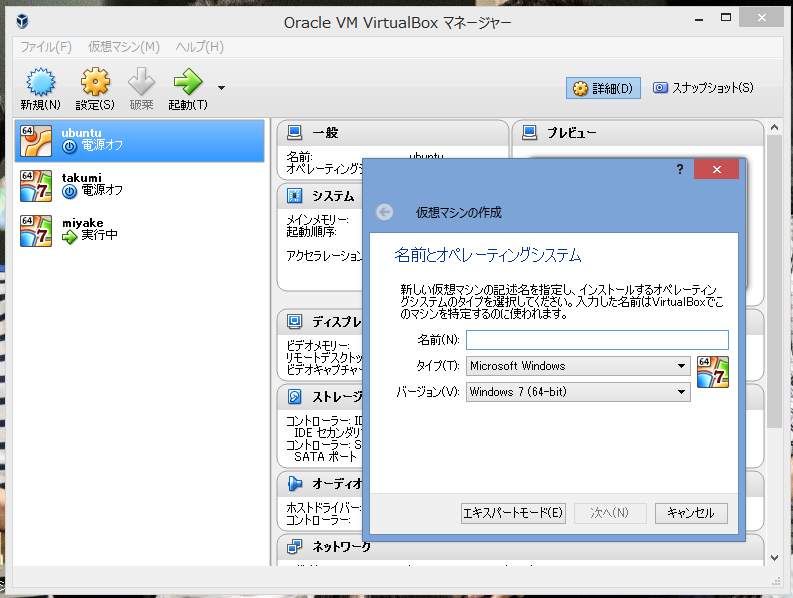
\includegraphics[width=15cm]{sinki.PNG}
\caption{ゲストマシンを作成}\label{サンプル図}
\end{figure}
ゲストマシンの名前,メモリサイズ,HDDの設定をする.


 \item 【設定(S)】を開き,ストレージをクリックし,ストレージツリーのコントローラー: IDE内の"空"を選択
\begin{figure}[H]
\centering
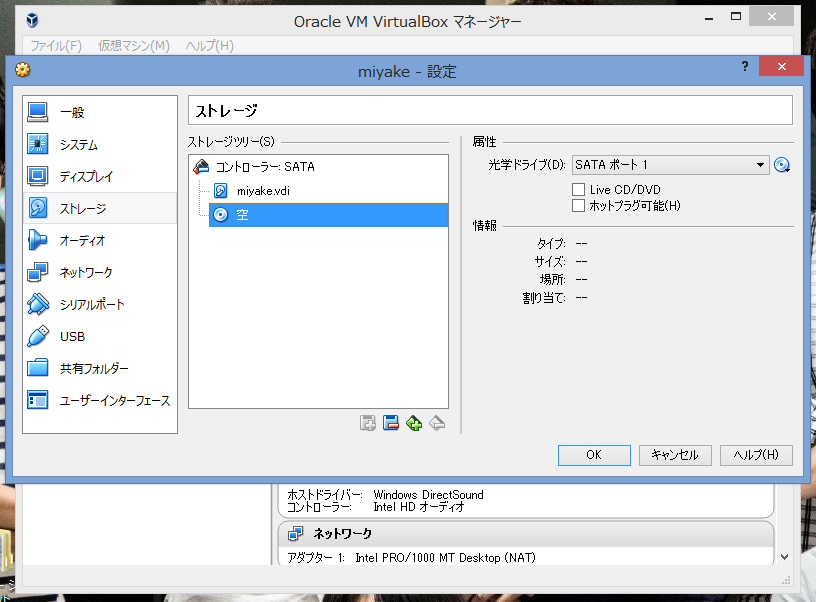
\includegraphics[width=15cm]{settei.PNG}
\caption{ストレージ設定画面}\label{サンプル図}
\end{figure}

  \item 属性内の一番右のディスクマークをクリックし,【仮想光学ディスクファイルを選択..】をクリックしてダウンロードしたISOイメージを選択

\begin{figure}[H]
\centering
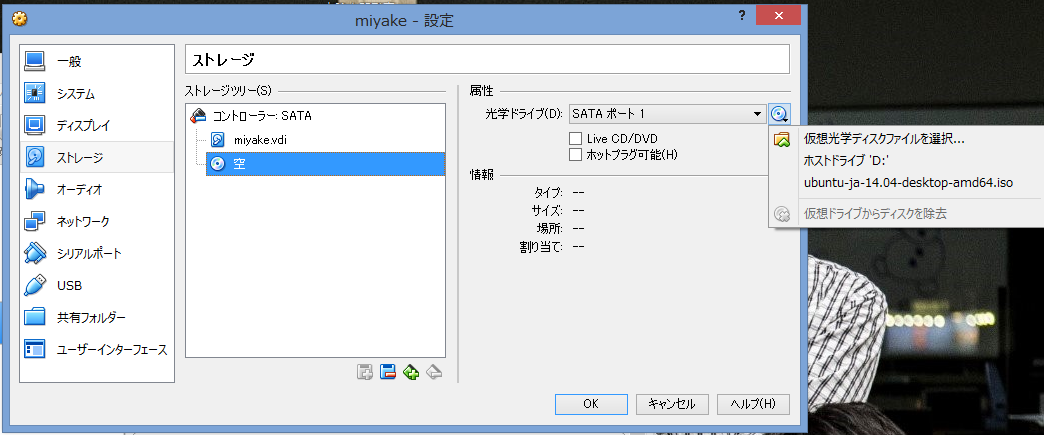
\includegraphics[width=15cm]{kasoukougaku.PNG}
\caption{仮想光学ディスクファイルの選択}\label{サンプル図}
\end{figure}
 

 \item 【OK】をクリックし,【起動(T)】を押してゲストマシンを起動
  \item Ubuntuをインストールと出るので,インストールをクリック


\begin{figure}[H]
\centering
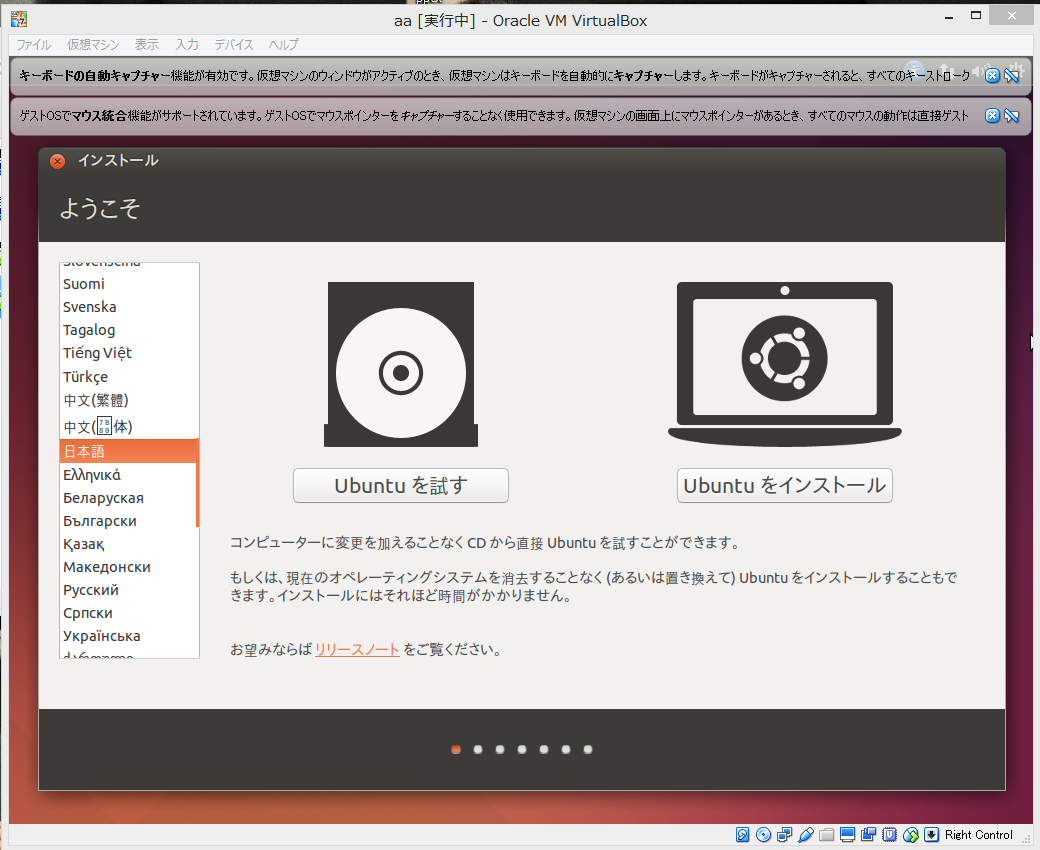
\includegraphics[width=15cm]{instal.PNG}
\caption{仮想光学ディスクファイルの選択}\label{サンプル図}
\end{figure}

  \item インストール完了したら,再起動と出るので再起動をクリック
 \item 起動して,国を選んだ後に,名前,パスワードを決めて完了
\end{enumerate}



\section{『Rubyによるクローラー開発技法の通りに株価を取得}


まずは,佐々木拓郎,るびきち『Rubyによるクローラー開発技法』(SBクリエイティブ, 2014)の5章14節の方法を参考にそのまま
実行してみる.

\subsection{端末を開く}

画面の一番左上にある,
マウスカーソルを乗せると「コンピュータとオンラインリソースを検索」と出るアイコンをクリック.

次に検索で「端末」と入力すると出てくるのでそれを使いコードを実行していく.
\begin{figure}[H]
\centering
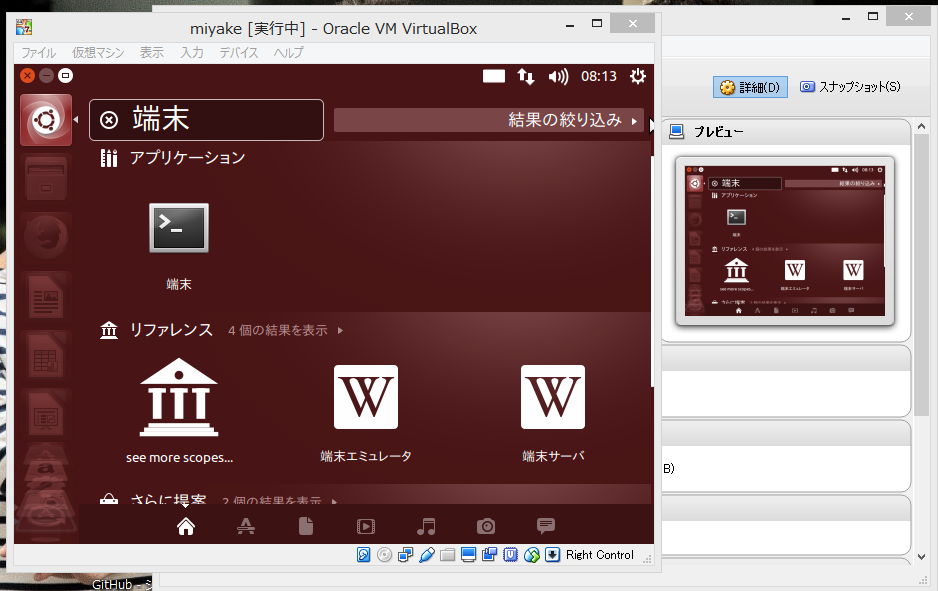
\includegraphics[width=15cm]{tanmatu.PNG}
\caption{端末の開き方}\label{サンプル図}
\end{figure}


\subsection{RubyとAnemoneをインストールする}

まずRubyのインストールをする.

sudo apt-get -y install ruby-dev libxml2-dev zlib1g-dev

\begin{figure}[H]
\centering
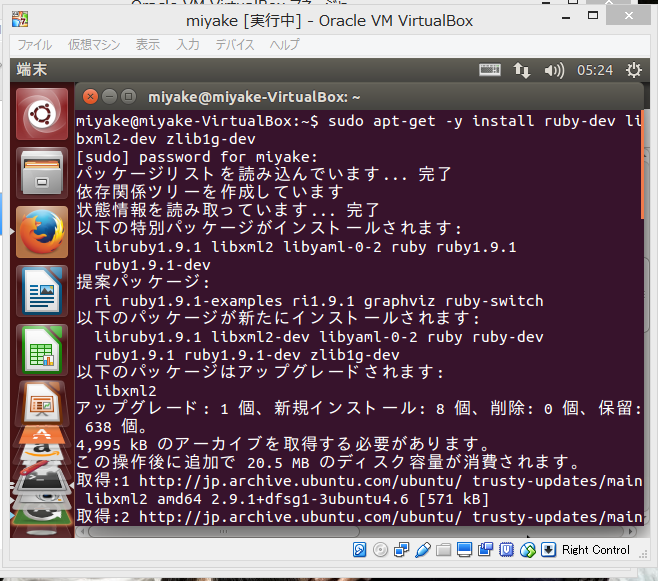
\includegraphics[width=15cm]{rubyins.PNG}
\caption{Rubyのインストール}\label{サンプル図}
\end{figure}


次に,Anemoneのインストールをする.
sudo gem install anemone

Anemoneとは
Webサイトを自動でクローリングするためのgemである.


\begin{figure}[H]
\centering
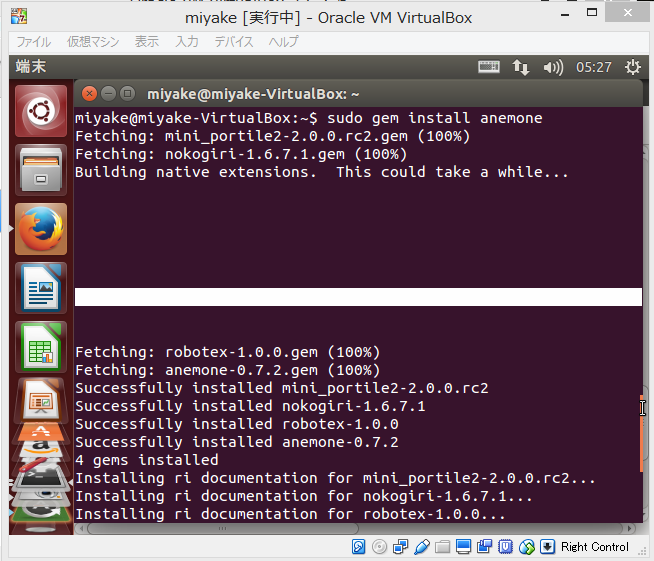
\includegraphics[width=15cm]{anemoneins.PNG}
\caption{Anemoneのインストール}\label{サンプル図}
\end{figure}




\subsection{作業ディレクトリを作り,移動する}

以下のコードで作業ディレクトリを作り,そのディレクトリに移動する.

mkdir ruby



cd ruby


\begin{figure}[H]
\centering
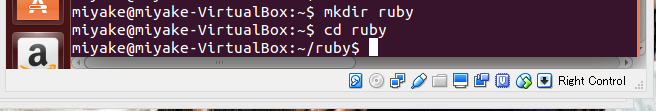
\includegraphics[width=15cm]{idou.PNG}
\caption{作業ディレクトリを作り,そのディレクトリに移動}\label{サンプル図}
\end{figure}

\subsection{サンプルスプリクトのダウンロードと使うファイルへの移動}
http://www.sbcr.jp/support/12019.html 
からサンプルスクリプトをダウンロードしてから先に進む.

【「Rubyによるクローラー開発技法」サンプルスクリプト】
をクリックするとダウンロードされる.

unzip ~/ダウンロード/RubyCrawlerSample.zip

でダウロードしたものを読み込む.

\begin{figure}[H]
\centering
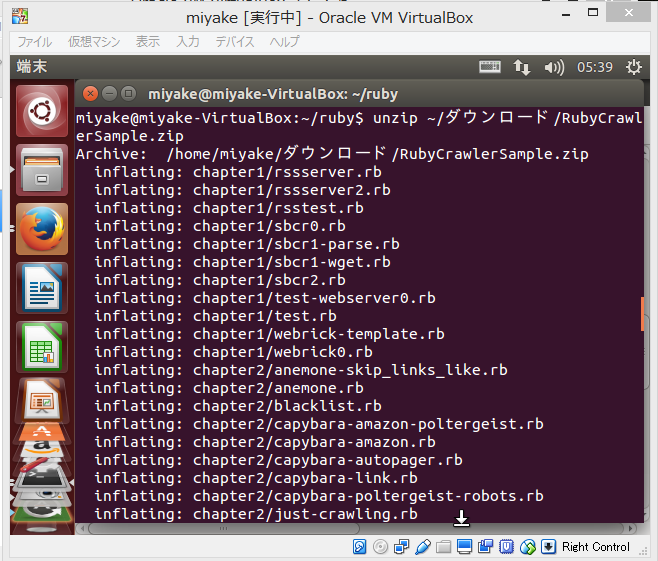
\includegraphics[width=15cm]{download.PNG}
\caption{ダウンロードファイルの読み込み}\label{サンプル図}
\end{figure}

cd chapter5

このコードで今回使うコードが入っている
chapter5に移動する.


\subsection{株価データを収集する}

ruby nokogiri-stock-history.rb

で株価を取得する.

これは本通りに進めているため,
ヤフーの株価を期間問わずに取得している.
\begin{figure}[H]
\centering
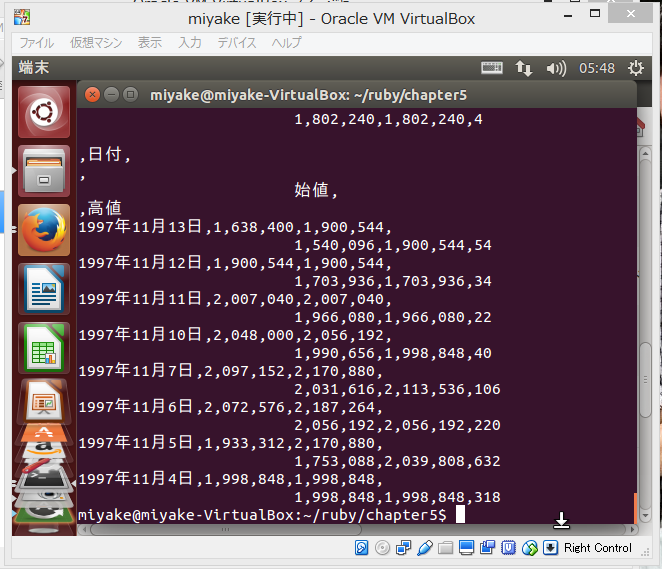
\includegraphics[width=15cm]{yahookabu.PNG}
\caption{ダウンロードファイルの読み込み}\label{サンプル図}
\end{figure}


左から,日付,始値,高値,安値,終値,出来高を表示している.

\subsection{株価取得コード}
ruby nokogiri-stock-history.rb

に書いてあるコードにより,ヤフーファイナンスから株価を取得するのだが,
そのコード(ヤフーファイナンスから1900年からこのコードを実行した日(最新のもの)までを取得するもの)は以下に記載する.

\begin{lstlisting}
# -*- coding: utf-8 -*-
require 'nokogiri'
require 'open-uri'

def get_nokogiri_doc(url)
	begin
		html = open(url)
	rescue OpenURI::HTTPError
		return
	end
	Nokogiri::HTML(html.read, nil, 'utf-8')
end

def has_next_page?(doc)
	doc.xpath("//*[@id='main']/ul/a").each {|element|
		return true if element.text == "次へ"
	}
	return false
end

def get_daily_data(doc)
	doc.xpath("//table[@class='boardFin yjSt marB6']/tr").each {|element|
		# 日付行および株式分割告知を回避
		if element.children[0].text != "日付" && element.children[1][:class] != "through"

		# 日付
		day = element.children[0].text

		# 始値
		open_price = element.children[1].text

		# 高値
		hight_price = element.children[2].text

		# 安値
		low_price = element.children[3].text

		# 終値
		closing_price = element.children[4].text

		# 出来高
		volume = element.children[5].text.gsub(/,/,'')

		puts "#{day},#{open_price},#{hight_price},
			#{low_price},#{closing_price},#{volume}"
		end
	}
end

# 証券コード
code="4689"

# 検索日
day=Time.now
ey=day.year
em=day.month
ed=day.day
start_url="http://info.finance.yahoo.co.jp/history/?
             sy=1900&sm=1&sd=1&ey=#{ey}&em=#{em}&ed=#{ed}&tm=d&code=#{code}"
num=1
puts "日付,始値,高値,安値,終値,出来高"
loop {
	url = "#{start_url}&p=#{num}"
	doc = get_nokogiri_doc(url)
	get_daily_data(doc)
	break if !has_next_page?(doc)
	num = num+1
}
		
\end{lstlisting}


\section{株価取得ツール使用方法}
本節では研究で開発した,株価取得の方法を書いていく.


\subsection{RubyとAnemoneのインストール}
第8章にある8.6.2と同じように進める.

もうすでに両方ともインストールしてあるため,入力は省略する.

\subsection{作業ディレクトリの作成と移動}

第8章にある8.6.3と同じように進めるが今回は名前を「kabuka」にして進める.

\begin{figure}[H]
\centering
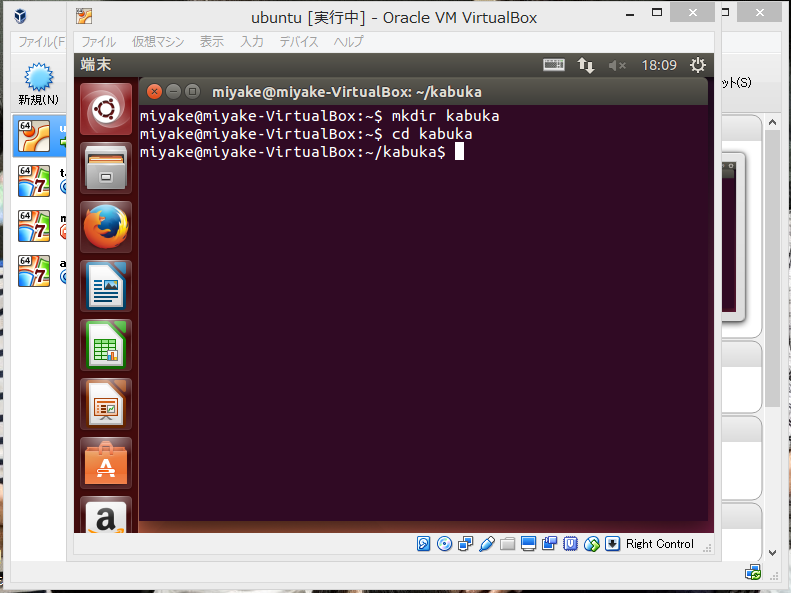
\includegraphics[width=15cm]{kabukaidou.PNG}
\caption{作業ディレクトリの作成と移動2}\label{サンプル図}
\end{figure}

\subsection{ディレクトリにコードファイルを入れる}



この3つのファイルを作成した「kabuka」のディレクトリに入れておく.
\begin{itemize}
  \item history.pl
  \item plot.sh
  \item nokogiri-stock-history2.rb
\end{itemize}



それぞれのコードとその役割を説明する.



「history.pl」は取得した株価データをどのようなグラフの描き方にするのかを決め,
そのグラフを描くものである.
\begin{lstlisting}
set datafile separator ","
set xdata time
set timefmt "%Y/%m/%d"
set format x "%Y/%m"
set xl "month"
set yl "price"
set terminal png
set out "stock.png"
plot 'stock.csv' using 1:2 with l linetype -1 title ""

\end{lstlisting}

「plot.sh」は取得した株価データをCSV形式に保存したり,
PNGファイルにするものである.
\begin{lstlisting}
rm -f stock.csv
cp $1.csv stock.csv

gnuplot history.pl

cp stock.png $1.png
rm -f stock.png

\end{lstlisting}

「nokogiri-stock-history2.rb」は銘柄・期間を指定し,株価をヤフーファイナンスから取得してくるものである.
\begin{lstlisting}
# -*- coding: utf-8 -*-
require 'nokogiri'
require 'open-uri'

def get_nokogiri_doc(url)
	begin
		html = open(url)
	rescue OpenURI::HTTPError
		return
	end
	Nokogiri::HTML(html.read, nil, 'utf-8')
end

def has_next_page?(doc)
	doc.xpath("//*[@id='main']/ul/a").each {|element|
		return true if element.text == "次へ"
	}
	return false
end

def get_daily_data(doc)
	doc.xpath("//table[@class='boardFin yjSt marB6']/tr").each {|element|
		# 日付行および株式分割告知を回避
		if element.children[0].node_name == "td" && element.children[1][:class] != "through"

		# 日付
		day = element.children[0].text.gsub(/年/,'/').gsub(/月/,'/').gsub(/日/,'')

		# 始値
		open_price = element.children[1].text.gsub(/,/,'')

		# 高値
		hight_price = element.children[2].text.gsub(/,/,'')

		# 安値
		low_price = element.children[3].text.gsub(/,/,'')

		# 終値
		closing_price = element.children[4].text.gsub(/,/,'')

		# 出来高
		volume = element.children[5].text.gsub(/,/,'')

		puts "#{day},#{open_price},#{hight_price},#{low_price},#{closing_price},#{volume}"
		end
	}
end


# 証券コード(コマンドライン引数)
code=ARGV[0]

# 検索日
sy=ARGV[1]
sm=ARGV[2]
sd=ARGV[3]
ey=ARGV[4]
em=ARGV[5]
ed=ARGV[6]
start_url="http://info.finance.yahoo.co.jp/history/?sy=#{sy}&sm=#{sm}&sd=#{sd}&ey=#{ey}&em=#{em}&ed=#{ed}&tm=d&code=#{code}"
num=1
puts "日付,始値,高値,安値,終値,出来高"
loop {
	url = "#{start_url}&p=#{num}"
	doc = get_nokogiri_doc(url)
	get_daily_data(doc)
	break if !has_next_page?(doc)
	num = num+1
}

\end{lstlisting}

\begin{figure}[htb]
\centering
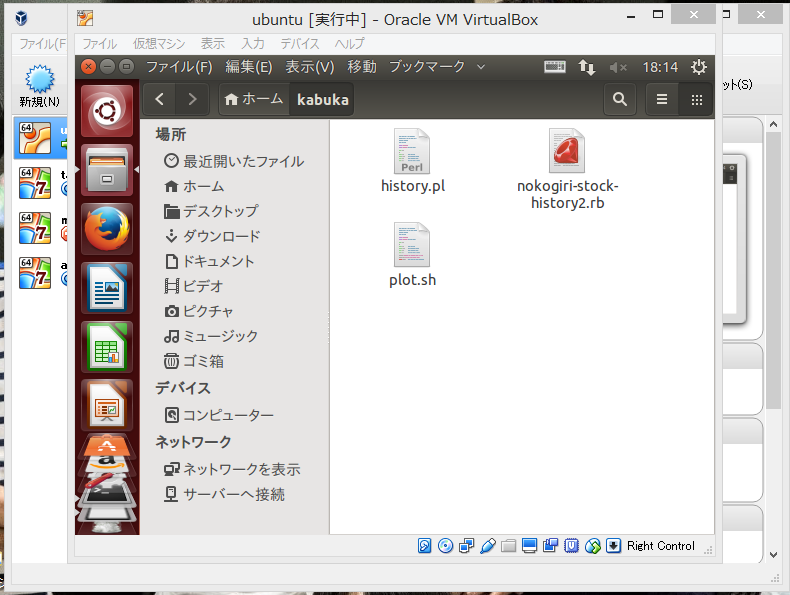
\includegraphics[width=15cm]{file.PNG}
\caption{ファイルを入れる}\label{サンプル図}
\end{figure}
{\small
\begin{verbatim}
これらのコードファイルが今回の研究成果となる,
株価データの可視化に使われるものである.






\section{ディレクトリのコードファイルを読み込む}

ls を実行すると以下のように読み取ることができる.

\begin{figure}[H]
\centering
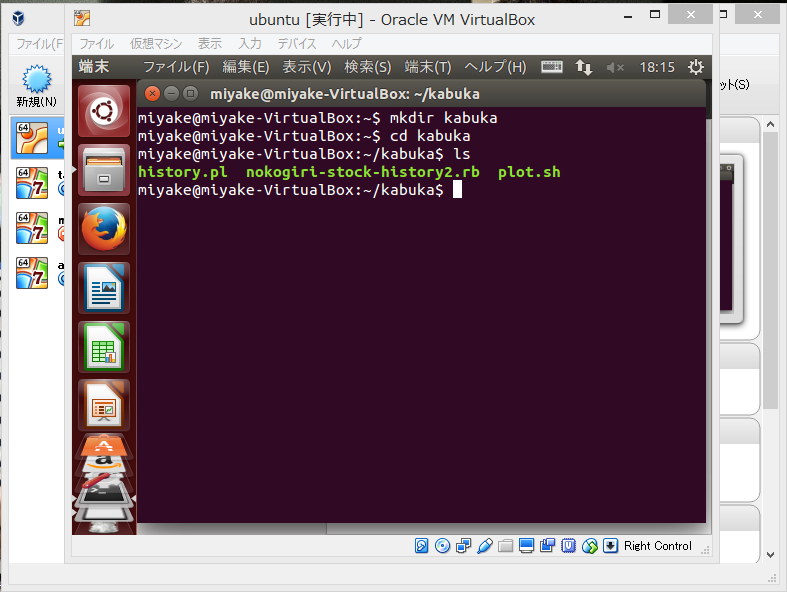
\includegraphics[width=15cm]{yomikomi.PNG}
\caption{ファイル読み込み}\label{サンプル図}
\end{figure}


\section{銘柄の選択}
今回はヤフーの株価を取得してみる.

銘柄コードは4689である.

\begin{figure}[H]
\centering
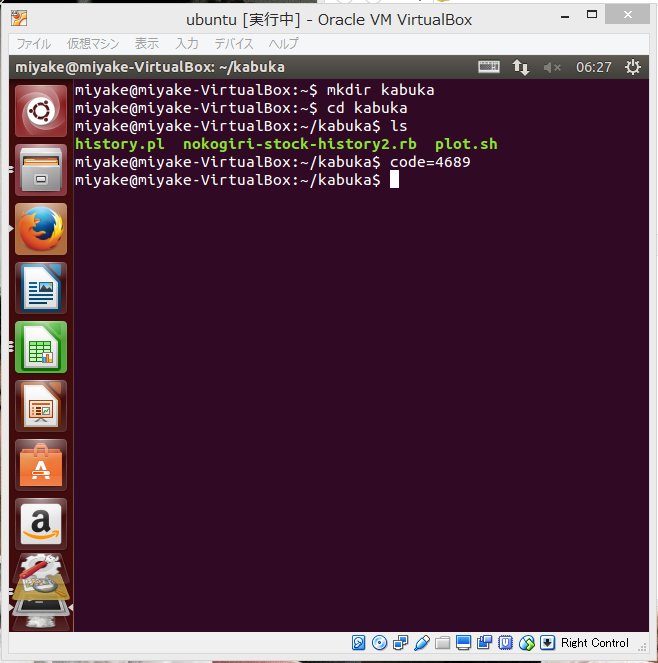
\includegraphics[width=15cm]{code.PNG}
\caption{銘柄選択}\label{サンプル図}
\end{figure}

code= 

イコールのあとに取得したい銘柄を入力するとその銘柄の株価を取得することができる.
\section{日付選択をし株価の取得}

\begin{figure}[H]
\centering
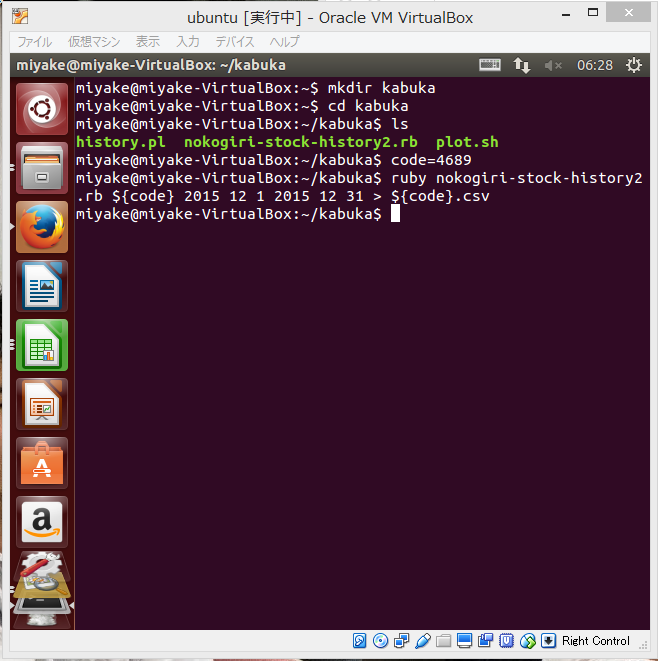
\includegraphics[width=15cm]{hiduke.PNG}
\caption{日付選択をし株価の取得}\label{サンプル図}
\end{figure}
{\small
\begin{verbatim}
ruby nokogiri-stock-history2.rb ${code} 2015 12 1 2015 12 31 > ${code}.csv

の ${code} 2015 12 1 2015 12 31 >${code}の中の数字を変えれば
日付を指定して株価を取得することができる.

\end{verbatim}
今回はヤフーの2015年12月1日から2015年12月31日までの株価を
取得する.



\subsection{Gnuplotをインストール}



まず,Gnuplotをインストールする.

「Gnuplot」は今回株価を描写するために必要なアプリケーションである.


\begin{figure}[H]
\centering
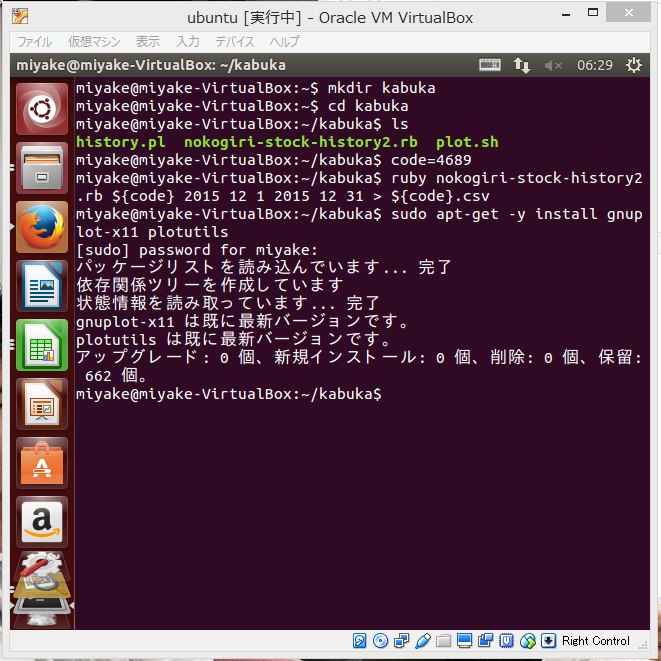
\includegraphics[width=15cm]{gnuplot.PNG}
\caption{Gnuplotのインストール}\label{サンプル図}
\end{figure}


sudo apt-get -y install gnuplot-x11 plotutils

このコードで「Gnuplot」をインストールすることができる.


\subsection{株価データの可視化}
株価データの可視化は取得した株価変動データをpngにして,
最初に作った「kabuka」のファイルに入れる.


\begin{figure}[H]
\centering
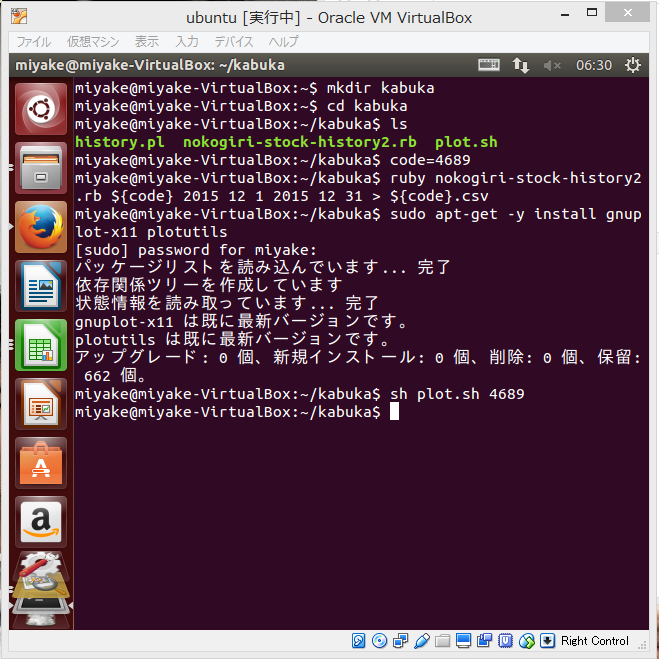
\includegraphics[width=15cm]{plot.PNG}
\caption{株価変動データをpngにする}\label{サンプル図}
\end{figure}

sh plot.sh 4689

を入力すると「4689.png」と「4689.csv」ができている.



\begin{figure}[H]
\centering
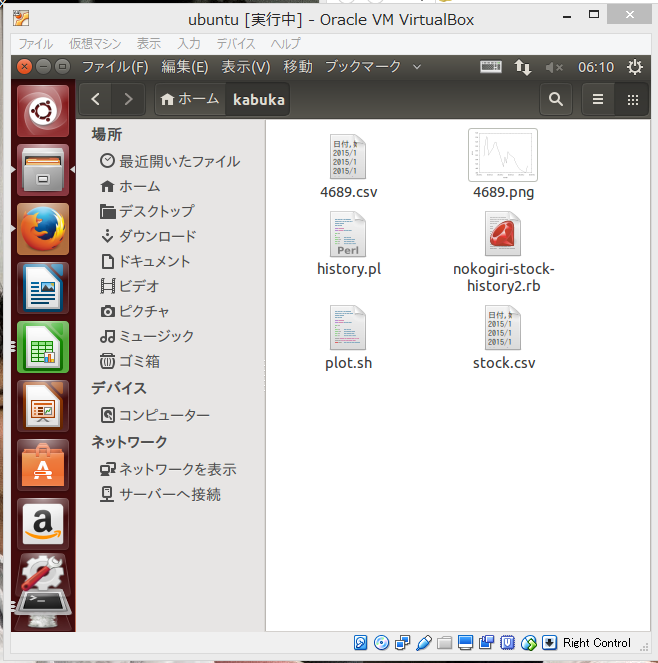
\includegraphics[width=15cm]{4689.PNG}
\caption{4689.png作成}\label{サンプル図}
\end{figure}

\subsection{描写した株価変動データ}

ヤフーの2015年12月1日から2015年12月31日までの株価変動データである.
以下のように株価を取得し,可視化をすることができる.
\begin{figure}[H]
\centering
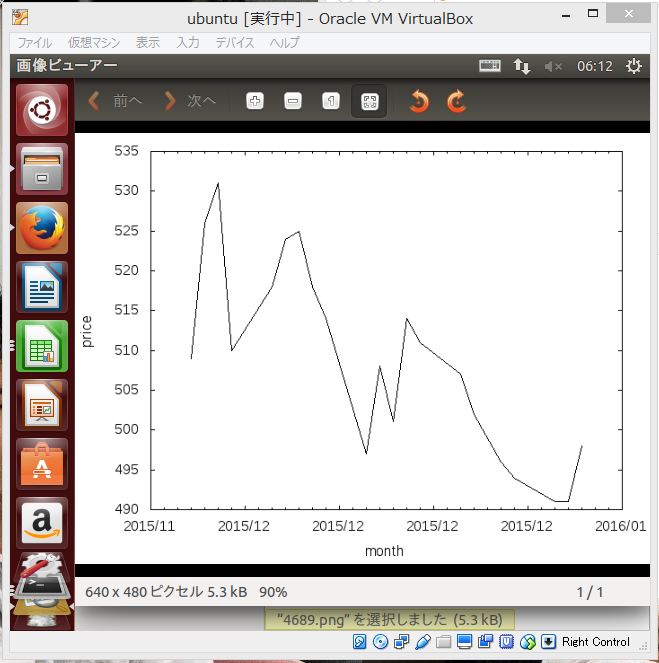
\includegraphics[width=15cm]{4689kasika.PNG}
\caption{ヤフーの株価変動}\label{サンプル図}
\end{figure}


日付と株価については「4689.csv」を開くと,
以下のように取得することができている.

\begin{figure}[H]
\centering
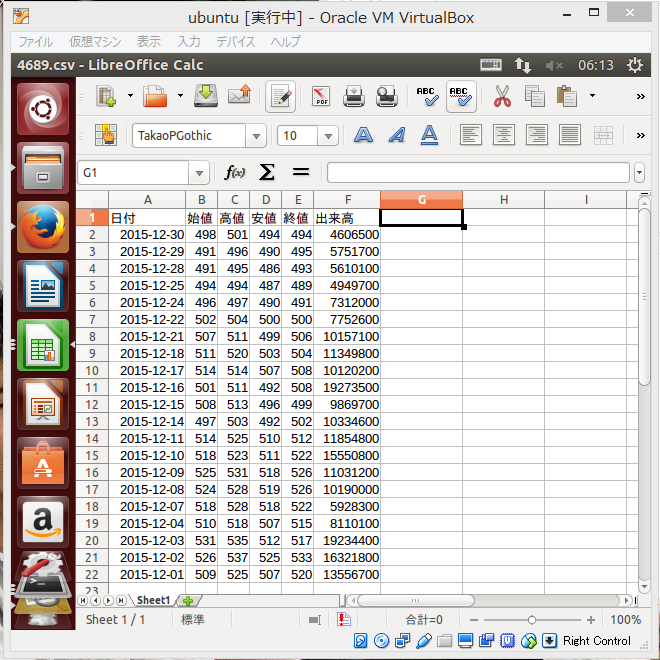
\includegraphics[width=15cm]{4689csv.PNG}
\caption{4689.csv}\label{サンプル図}
\end{figure}



\section{背景にある調査の進め方}
背景にある調査はどんな事故や事例でも進められるものではなく,
チャレンジャー号墜落事故の事例と同じような条件の事故を調べる.



\subsection{調べる事故の条件}
\begin{itemize}
  \item 複数の企業が関わっていること
  \item 原因企業が判明するまでに時間がかかっていること
  \item 原因企業が株式会社であること

\end{itemize}


\subsection{条件に当てはまる事故}
ウェブ検索で見つかった事故は以下の4件である.
\begin{itemize}
  \item スペースシャトル・チャレンジャー号爆発事故

1986年1月28日,アメリカ合衆国のスペース・シャトルチャレンジャー号が射ち上げから73秒後に分解し,7名の乗組員が死亡した事故である.同オービタは北米東部標準時午前11時39分(16:39UTC,1月29日1:39JST)にアメリカ合衆国フロリダ州中部沖の大西洋上で空中分解した.

<事故の概略>

機体全体の分解は,右側固体燃料補助ロケット(Solid Rocket Booster, SRB)の密閉用Oリングが発進時に破損したことから始まった.Oリングの破損によってそれが密閉していたSRB接続部から漏洩が生じ,固体ロケットエンジンが発生する高温・高圧の燃焼ガスが噴き出して隣接するSRB接続部材と外部燃料タンク(External Tank, ET)に悪影響を与えた.この結果,右側SRBの尾部接続部分が分離すると共に外部燃料タンクの構造破壊が生じた.空気力学的な負荷により軌道船は一瞬の内に破壊された\cite{bakuhatuziko}.

\begin{figure}[H]
\centering
\includegraphics[width=15cm]{challenger_explosion.PNG}
\caption{チャレンジャー号爆発」}\label{サンプル図}
\end{figure}


  \item トルコ航空DC-10パリ墜落事故

1974年にフランスで発生したトルコ航空981便のDC-10-10(マクドネルダグラス社製,機体記号TC-JAV)が墜落した航空事故である(別名:トルコ航空981便墜落事故).

<事故の概略>

事故機は離陸10分後,,パリから北へ15km離れたサン=パトゥス村 (Saint-Pathus) 上空、高度11500フィート(3500メートル)まで上昇したときに,ロックが不完全だった左側後部貨物室ドアが客室の与圧により吹き飛ばされて急減圧が起こった.この時にパイロットが持っていたマニュアルが壁にたたきつけられる音がコックピットボイスレコーダーに収録されている.貨物室の減圧に伴い客室の床が破壊され,乗客6名が座席ごと空中に放り出された.また,床下を通るコントロールラインが切断されて,方向舵,昇降舵,尾部エンジンの制御が不可能になり,操縦不能のままドアの脱落から1分17秒後に430ノット(約796km/h)の速さで墜落に至った\cite{toruko}.


\begin{figure}[H]
\centering
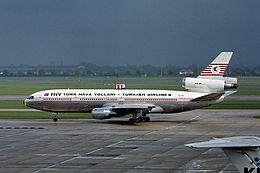
\includegraphics[width=15cm]{260px-McDonnell_Douglas_DC-10-10,_Turkish_Airlines_AN1815013.PNG}
\caption{トルコ航空DC-10」}\label{サンプル図}
\end{figure}


  \item 日本航空123便墜落事故

1985年(昭和60年)8月12日月曜日18時56分に,東京(羽田)発大阪(伊丹)行同社定期123便ボーイング747SR-100(ジャンボジェット,機体記号JA8119,製造番号20783)が,群馬県多野郡上野村の高天原山の尾根(通称「御巣鷹の尾根」)に墜落した航空事故である.

<事故の概略>      

事故機の後部圧力隔壁が損壊し,その損壊部分から客室内の空気が機体後部に流出したことによって,機体尾部と垂直尾翼の破壊が起こった.さらに、4系統ある油圧パイプがすべて破壊されたことで作動油が流出し,操縦機能の喪失が起こった\cite{nihon}.

\begin{figure}[H]
\centering
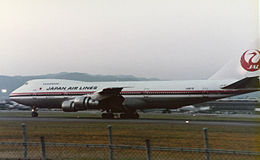
\includegraphics[width=15cm]{JA8119_at_Itami_Airport_1984.PNG}
\caption{日本航空123便」}\label{サンプル図}
\end{figure}


  \item 東京航空交通管制システム障害

2003年3月1日7時ごろ,飛行計画情報処理システム(FDP)のシステムトラブルは,航空会社の欠航便205便,30分以上の遅延便は1462便,また2日間にわたってダイヤが乱れるという大障害となった.

<障害の概略>
 
2002年9月に変更したFDPにNEC(日本電気(株))によるプログラム・ミスがあった.
2003年3月1日,「防衛庁システム対応プログラム」を変更したことと,当日7時,オンライン情報処理プログラムが起動したことにより,これまで隠れていたこのミスが表に現れ,システムがダウンした\cite{kouku}.

\end{itemize}

\subsection{各事故に関連する企業情報の入手}

事故の原因企業以外にも事故に関連する企業情報を取得することができないと,
比較対象がないため,調査を進めることができない.

本研究ではその技術の開発を目的とはしていないため,これより先は進めることができない.



\subsection{事故関連企業の株価変動データの比較・解析}
事故関連企業の株価変動データの比較・解析を行う.

この流れを事故事例を増やして行っていく.










\section{横浜マンション傾斜問題の調査}
開発したツールを使い株価変動データをいくつか比較できるかテストする.

それと同時に背景にあることを調査するための条件に当てはまる事例が「横浜マンション傾斜問題」であり,
関連する企業も公になっているためこの事例について調査する.



\subsection{横浜マンション傾斜問題とは}
この問題は2015年10月14日新聞報道があって話題になった.

三井不動産レジデンスが横浜市に,2006(平成18)年から販売が開始されたマンション,「パークシティLaLa横浜」の
タイルを積んだ際にできる継ぎ目である「目地」が上下で最大2.4cmずれていたという問題である.



\subsection{横浜マンション傾斜理由}
マンション傾斜の理由は10月14日,新聞報道があった後に下請けであった「旭化成建材」が杭打ちのデータ改ざんを認めた.
本来使うはずであった杭より短いものを使っていたため,マンションが傾いてしまった.

だが,短い杭を意図的に発注したのは「三井住友建設」である.
\subsection{横浜マンション建設の流れ}
「パークシティLaLa横浜」の建設の流れは以下のとおりである.

\begin{enumerate}
  \item 三井不動産レジデンシャルが工事発注をする
  \item 元請けとして三井住友建設が入る
  \item 1次下請けとして日立ハイテクノロジーズが入る
  \item 2次下請けとして旭化成建材が入る
\end{enumerate}

このような流れからこのマンションは建てられた.

\subsection{次々と発覚する事実}
この問題は次々と事実が発覚していった.

2015年10月14日に三井不動産がマンションが傾いていることを公表した.

公表当日には旭化成建材が杭打ちのデータ改ざんを認めた.


2015年10月24日三井住友建設には,施工主の三井住友建設が,杭の長さが足りないとが判明した場所の強固な地盤「支持層」が
実際には深さ16メートル付近にあるのに,設計段階で2メートル浅い約14メートルと見込んでくいを発注していたことが取材により発覚した.

さらには,
2015年10月27日に日立ハイテクノロジーズが
問題があった場合の責任は2次下請けが負うとの契約を結んでいたという.

「技術的な知見はなく,旭化成建材の担当者が改ざんした工事データの「信憑性は判断できなかった」と旭化成建材に丸投げをした疑惑が残った.


\subsection{原因企業}

前節の各企業で主犯であったのは元請けである三井住友建設であると考える.

なぜなら2メートル短い杭を発注し,下請けである旭化成建材にそのまま建設をさせたからである.

そのことを前提としてこの事例に関連する4社の株価を取得していく.

\chapter{結果}
「横浜マンション傾斜問題」の関連企業の株価を取得した結果を書いていく.


section{株価の可視化}
\subsection{三井不動産}

株価変動データは以下のようであった.


\begin{figure}[H]
\centering
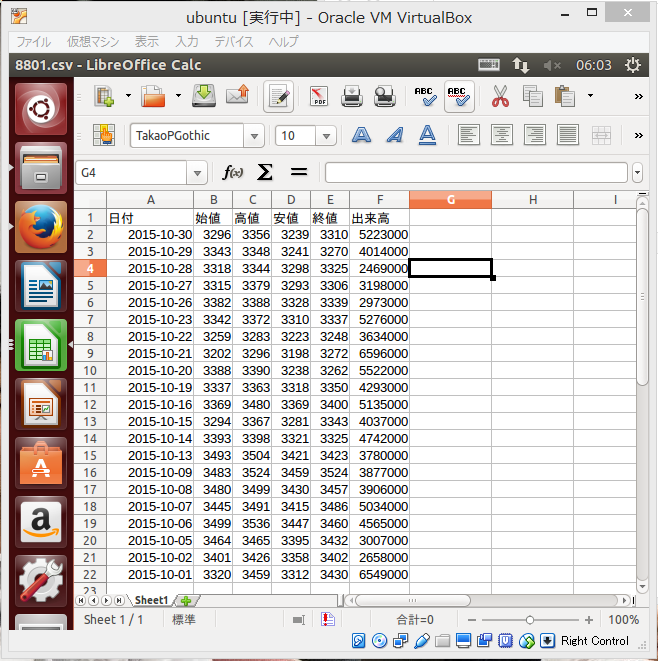
\includegraphics[width=15cm]{8801csv.PNG}
\caption{三井不動産株価変動}\label{サンプル図}
\end{figure}


グラフにより可視化したのは以下のものである.




\begin{figure}[H]
\centering
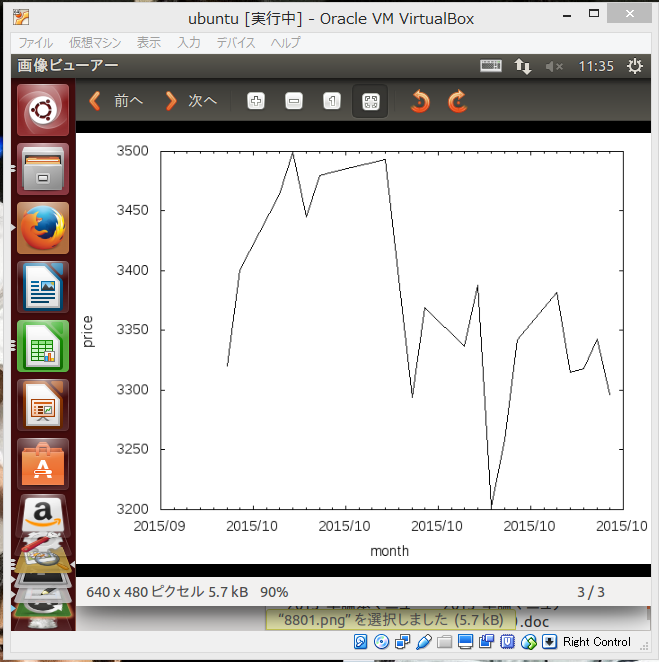
\includegraphics[width=15cm]{8801.PNG}
\caption{三井不動産株価変動グラフ}\label{サンプル図}
\end{figure}




\section{旭化成}



株価変動データは以下のようであった.


\begin{figure}[H]
\centering
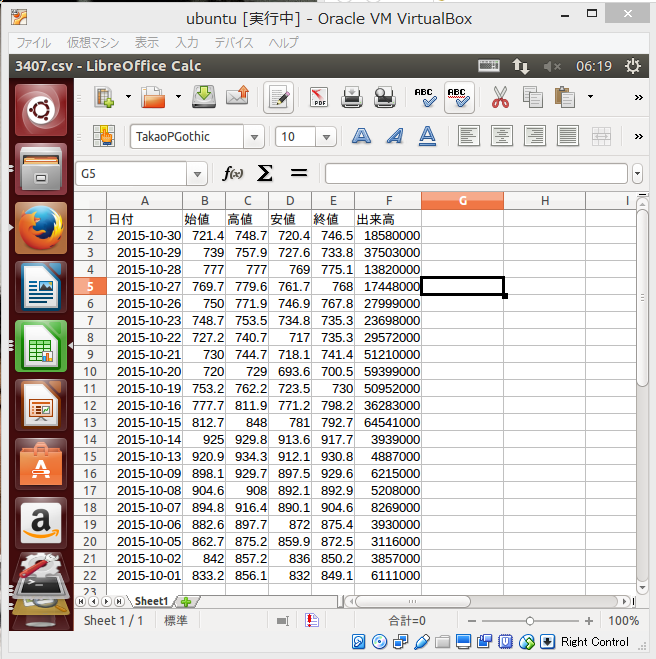
\includegraphics[width=15cm]{3407csv.PNG}
\caption{旭化成株価変動}\label{サンプル図}
\end{figure}


グラフにより可視化したのは以下のものである.




\begin{figure}[H]
\centering
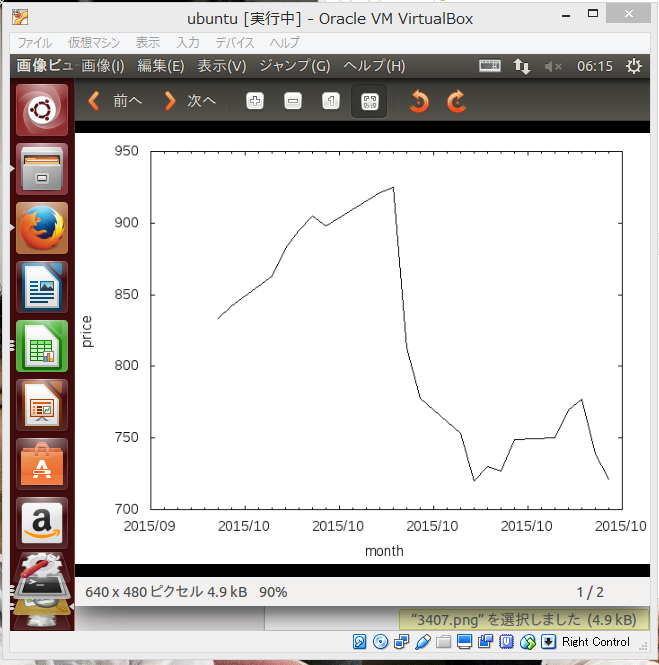
\includegraphics[width=15cm]{3407.PNG}
\caption{旭化成株価変動グラフ}\label{サンプル図}
\end{figure}




\section{三井住友建設}

株価変動データは以下のようであった.


\begin{figure}[H]
\centering
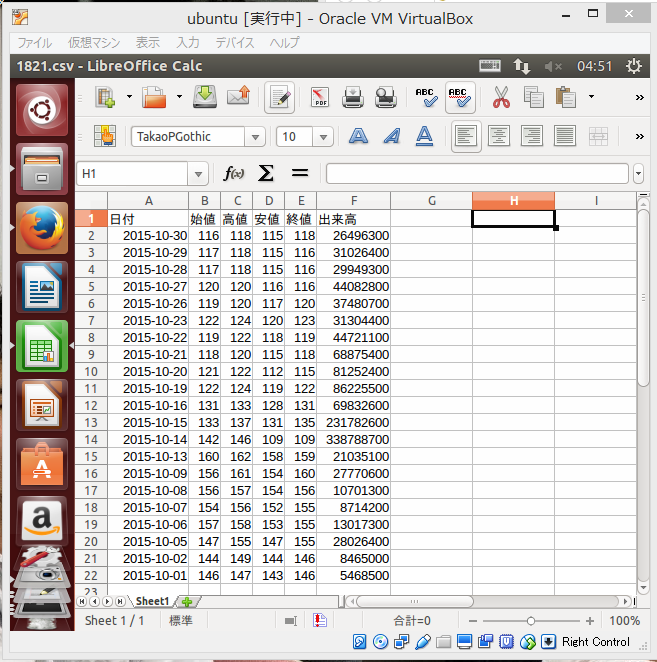
\includegraphics[width=15cm]{1821csv.PNG}
\caption{三井住友建設株価変動}\label{サンプル図}
\end{figure}


グラフにより可視化したのは以下のものである.




\begin{figure}[H]
\centering
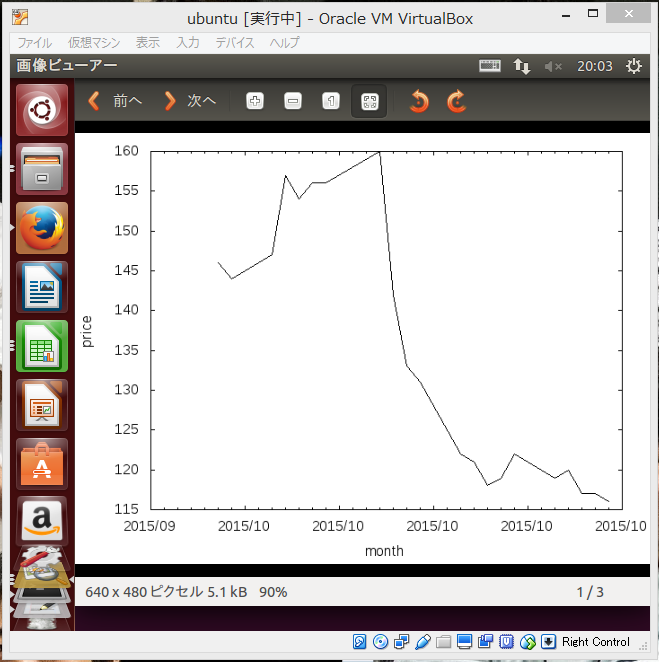
\includegraphics[width=15cm]{1821.PNG}
\caption{三井住友建設株価変動グラフ}\label{サンプル図}
\end{figure}




\section{日立ハイテクノロジーズ}

株価変動データは以下のようであった.


\begin{figure}[H]
\centering
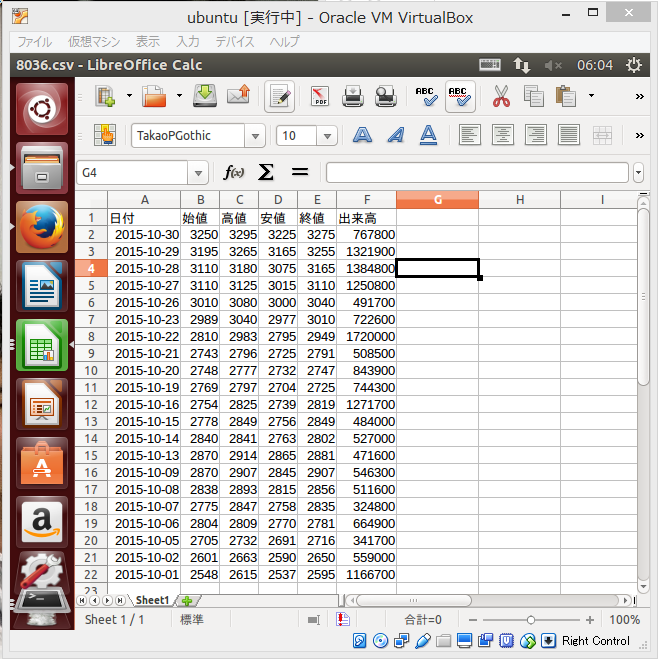
\includegraphics[width=15cm]{8036csv.PNG}
\caption{日立ハイテクノロジーズ株価変動}\label{サンプル図}
\end{figure}


グラフにより可視化したのは以下のものである.




\begin{figure}[H]
\centering
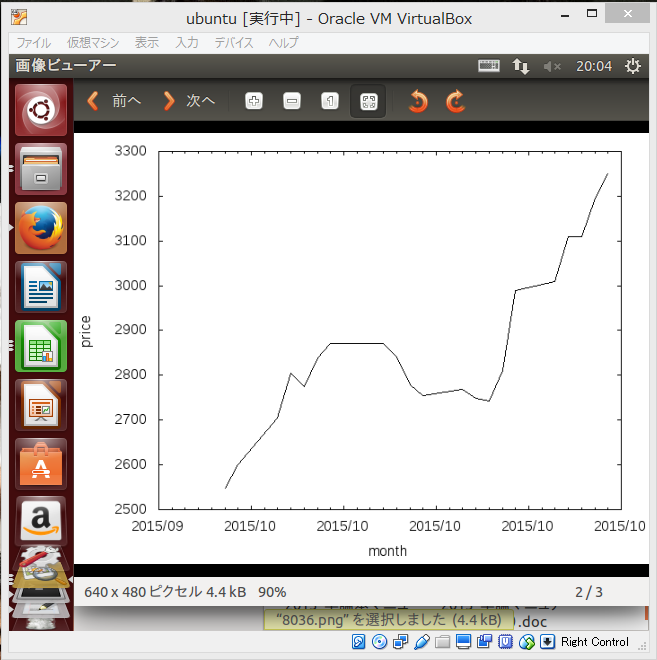
\includegraphics[width=15cm]{8036.PNG}
\caption{日立ハイテクノロジーズ株価変動グラフ}\label{サンプル図}
\end{figure}


section{株価変動の結果}

関連企業の株価変動結果は以下の通りであった.
\begin{itemize}
  \item 三井不動産は13日から下がり始め,14日は2パーセント下落
  \item 旭化成は10月14日まで変動はなく,15日の始値は14日の終値から11.4パーセント下落
  \item 三井住友建設は13日終値から14日始値は12パーセント下落し,14日始値と終値で30パーセント下落,その後持ち直さなかった
  \item 日立ハイテクノロジーズはトレンドを乱すことなく,特に変化なし
\end{itemize}

\chapter{考察}
株価に変動があったのは日立ハイテクノロジーズ以外の3社である.

旭化成は14日に杭打ちデータ改ざんを認めたため株価が下がるのは当たり前であると考える.

だが三井住友建設は10月24日に短い杭を8流していたことを認めたのにもかかわらず,
14日に大幅にトレンドが乱れ下落している.
この結果を見る限り,株式市場は三井住友建設が主犯であると言っているように感じられる.


さらにこの調査を進めるためには,背景にある事故条件とマッチする事故・事例を増やし,
その事故・事例に関連する企業の情報を取得する技術を確立していかないといけないと考える.

Rubyによるクローラー開発技法により,今回であれば取得したい銘柄の株価を期間を指定して取得することができた.
それができたということは,何か調べ物をしたりするときにはクローラー開発ができれば,
ネット上にある膨大な情報の中から自分の取得したい情報のみが取得できると考える.


\chapter{結論}
本研究の目的である株価取得とその可視化は成功し,いくつかの企業の株価変動データの比較もできるようになった.

背景の調査に関してはマンション傾斜の事例だけを見れば株式市場は三井住友建設が今回の主犯であったとマスメディアより早く特定ができていたと言えるが,事例が1つしかないため断言はできない.
開発したツールを使い,事例を増やし研究していけば背景にある調査はさらに進められる.


\bibliographystyle{junsrt}
\bibliography{biblio}%「biblio.bib」というファイルが必要.

\end{document}